\documentclass[12pt]{amsproc}
\newcommand{\course}{Ring and module theory}
\input{mystuff}

%\usepackage{mathptmx}
%\usepackage{newtxtext}

%\usepackage{xcolor,etoolbox}
%\definecolor{mymagenta}{RGB}{195,51,117} % magenta
%\definecolor{myblue}{RGB}{46,118,181} % blue
% \definecolor{mydarkblue}{RGB}{36,43,95} % dark blue
%\definecolor{mygreen}{RGB}{79,122,59} % green
% \definecolor{midnight}{RGB}{40,104,145} % midnight blue

% \AtBeginEnvironment{theorem}{\color{myblue}}
% \AtEndEnvironment{theorem}{\color{black}}
% \AtBeginEnvironment{definition}{\color{mymagenta}}
% \AtEndEnvironment{definition}{\color{black}}
% \AtBeginEnvironment{proof}{\color{mydarkblue}}
% \AtEndEnvironment{proof}{\color{black}}
%\AtBeginEnvironment{exercise}{\color{mygreen}}
%\AtEndEnvironment{exercise}{\color{black}}
%\AtBeginEnvironment{example}{\color{mymagenta}}
%\AtEndEnvironment{example}{\color{black}}

% \AtBeginEnvironment{proposition}{\color{myblue}}
% \AtEndEnvironment{proposition}{\color{black}}

%\usetikzlibrary{positioning}
\usetikzlibrary{arrows,positioning,shapes}


\begin{document}

\begin{abstract}
    The notes correspond to the bachelor 
    course \textbf{Ring and Module Theory} (2024) of the 
    Vrije Universiteit Brussel, 
    Faculty of Sciences, 
    Department of Mathematics and Data Sciences. 
\end{abstract}

\maketitle

\setcounter{tocdepth}{1}
\tableofcontents 


\begin{figure}[h]
    \includegraphics[scale=0.2]{VUB.jpg}
\end{figure}


\include{introduction}
\thispagestyle{plain}
\begin{center}
    \color{green!30!black}\textbf{List of topics}
\end{center}
\bigskip 

\contentsline {section}{\tocsubsection {\S }{1.1}{Rings}}{4}{subsection.1.1}%
\contentsline {section}{\tocsubsection {\S }{1.2}{Ideals}}{6}{subsection.1.2}%
\contentsline {section}{\tocsubsection {\S }{1.2}{Quotients}}{6}{subsection.1.2}%
\contentsline {section}{\tocsubsection {\S }{2.1}{The Chinese remainder theorem}}{13}{subsection.2.1}%
\contentsline {section}{\tocsubsection {\S }{3.1}{Noetherian rings}}{17}{subsection.3.1}%
\contentsline {section}{\tocsubsection {\S }{3.2}{Factorization}}{19}{subsection.3.2}%
\contentsline {section}{\tocsubsection {\S }{5.1}{Zorn's lemma}}{30}{subsection.5.1}%
\contentsline {section}{\tocsubsection {\S }{5.2}{The characteristic of a ring}}{33}{subsection.5.2}%
\contentsline {section}{\tocsubsection {\S }{5.3}{Group algebras}}{34}{subsection.5.3}%
\contentsline {section}{\tocsubsection {\S }{6.1}{Group representations}}{36}{subsection.6.1}%
\contentsline {section}{\tocsubsection {\S }{7.1}{Characters}}{43}{subsection.7.1}%
\contentsline {section}{\tocsubsection {\S }{7.2}{Schur's orthogonality relations}}{45}{subsection.7.2}%
\contentsline {section}{\tocsubsection {\S }{8.1}{Examples}}{51}{subsection.8.1}%
\contentsline {section}{\tocsubsection {\S }{8.2}{Finite simple groups (optional)}}{55}{subsection.8.2}%
\contentsline {section}{\tocsubsection {\S }{9.1}{Modules}}{59}{subsection.9.1}%
\contentsline {section}{\tocsubsection {\S }{10.1}{Noetherian modules}}{65}{subsection.10.1}%
\contentsline {section}{\tocsubsection {\S }{10.2}{Quotient fields}}{67}{subsection.10.2}%
\contentsline {section}{\tocsubsection {\S }{10.3}{Free modules}}{68}{subsection.10.3}%
\contentsline {section}{\tocsubsection {\S }{11.1}{Modules over principal domains}}{74}{subsection.11.1}%
\contentsline {section}{\tocsubsection {\S }{12.1}{Smith's normal form}}{78}{subsection.12.1}%


\chapter{}

\section*{Rings}

We will devote five lectures to basic theory of rings. The topics to cover are:
1) Basic definitions and examples, 2) ideals, homomorphisms and quotient rings,
3) Chinese remainder theorem, 
4) noetherian rings and Hilbert's theorem, 
5) factorization in commutative rings, 
6) Fermat's theorem, and 
7) Zorn's lemma and maximal ideals. 

\begin{definition}
\index{Ring}
A \textbf{ring} is a set $R$ with two binary operations, the addition
$R\times R\to R$, $(x,y)\mapsto x+y$, and the multiplication
$R\times R\to R$, $(x,y)\mapsto xy$, such that
the following properties hold:
\begin{enumerate}
    \item $(R,+)$ is an abelian group.
    \item $(xy)z=x(yz)$ for all $x,y,z\in R$.
    \item $x(y+z)=xy+xz$ for all $x,y,z\in R$.
    \item $(x+y)z=xz+yz$ for all $x,y,z\in R$.
    \item There exists $1_R\in R$ such that $x1_R=1_Rx=x$ for all $x\in R$.
\end{enumerate}
\end{definition}

Our definition of a ring is that of a ring with identity. In general one
writes the identity element $1_R$ as $1$ if there is no risk of confusion.

\begin{definition}
\index{Ring!commutative}
A ring $R$ is said to be \textbf{commutative} if $xy=yx$ for all $x,y\in R$. 
\end{definition}

\begin{example}
$\Z$, $\Q$, $\R$ and $\C$ are commutative rings.
\end{example}

\begin{example}
    The set  
    \[
    \R[X]=\left\{\sum_{i=0}^na_iX^i:n\in\N_0,\,a_1,\dots,a_n\in \R\right\}
    \]
    of real polynomials in one variable 
    is a commutative ring with the usual operations. 
\end{example}

More generally, if $R$ is a commutative ring, then $R[X]$ is a commutative ring. This construction
allows us to define 
the polynomial ring $R[X,Y]$ in two commuting variables $X$ and $Y$ and coefficients in $R$ as 
$R[X,Y]=(R[X])[Y]$. One can also define the ring  
$R[X_1,\dots,X_n]$ of real polynomials 
in $n$ commuting variables $X_1,\dots,X_n$ with coefficients in $R$ as 
$R[X_1,\dots,X_n]
=(R[X_1,\dots,X_{n-1}])[X_n]$.

\begin{example}
    If $A$ is an abelian group, then 
    the set 
    $\End(A)$ of group homomorphisms $A\to A$ is a ring with
    \[
    (f+g)(x)=f(x)+g(x),\quad
    (fg)(x)=f(g(x)),\quad f,g\in\End(A)\text{ and }x\in A.
    \]
\end{example}

Let $R$ be a ring. 
Some facts:
\begin{enumerate}
    \item $x0=0x=x$ for all $x\in R$.
    \item $x(-y)=-xy$ for all $x,y\in R$.
    \item If $1=0$, then $|R|=1$. 
\end{enumerate}

\begin{example}
    The real vector space $H(\R)=\{a1+bi+cj+dk:a,b,c,d\in\R\}$ with basis $\{1,i,j,k\}$ 
    is a ring with the multiplication induced by
    the formulas 
    \[
    i^2=j^2=k^2=-1,
    \quad ij=k,
    \quad jk=i,
    \quad ki=j.
    \]
    As an example, let us perform a calculation in $H(\R)$: 
    \[
    (1+i+j)(i+k)=i+k-1+ik+ji+jk=i+k-1-j-k+i=-1+2i-j,
    \]
    as $ij=i(ij)=-j$. This is the ring of real \textbf{quaternions}.
\end{example}

\begin{example}
    Let $n\geq2$. 
    The abelian group $\Z/n=\{0,1,\dots,n\}$ of integers modulo $n$ is a ring 
    with the usual multiplication modulo $n$. 
\end{example}

\begin{example}
    Let $n\geq1$. 
    The set $M_n(\R)$ of real $n\times n$ matrices is a ring with the usual matrix operations. Recall
    that if $a=(a_{ij})$ and $b=(b_{ij})$, the multiplication $ab$ is given by
    \[
    (ab)_{ij}=\sum_{k=1}^n a_{ik}b_{kj}.
    \]
\end{example}

Similarly, for any ring $R$ one defines the ring $M_n(R)$ of $n\times n$ matrices
with coefficients in $R$. 

\begin{definition}
\index{Subring}
    Let $R$ be a ring. A \textbf{subring} $S$ of $R$ is a subset $S$ such that
    $(S,+)$ is a subgroup of $(R,+)$ such that $1\in S$ and 
    if $x,y\in S$, then $xy\in S$. 
\end{definition}

Clearly, $\Z\subseteq\Q\subseteq\R\subseteq\C$ is a chain of subrings. 

\begin{example}
    \index{Gauss integers}
    $\Z[i]=\{a+bi:a,b\in\Z\}$ is a subring of $\C$. 
    This is known as the ring of \textbf{Gauss integers}.  
\end{example}

\begin{example}
    $\Q[\sqrt{2}]=\{a+b\sqrt{2}:a,b\in\Q\}$ is a subring of $\R$. 
\end{example}

\begin{example}
    \index{Center!of ring}
    If $R$ is a ring, then the \textbf{center} 
    $Z(R)=\{x\in R:xy=yx\text{ for all $y\in R$}\}$ 
    is a subring of $R$. 
\end{example}

If $S$ is a subring of a ring $R$, then the zero element 
of $S$ is the zero element of $R$, i.e. $0_R=0_S$. Moreover, 
the additive inverse of an element $s\in S$ 
is the additive inverse of $s$ as an element of $R$. 	

\begin{exercise}\
\begin{enumerate}
	\item If $S$ and $T$ are subrings of $R$, then $S\cap T$ is a subring of $R$.
	\item If $R_1\subseteq R_2\subseteq\cdots$ is a sequence of subrings of $R$, then 
	$\cup_{i\geq1}R_i$ is a subring of $R$. 
\end{enumerate}
\end{exercise}

\begin{definition}
\index{Units}
	Let $R$ be a ring. An element $x\in R$ is 
	a \textbf{unit} if there exists $y\in R$ such that $xy=yx=1$. 
\end{definition}

The set $\mathcal{U}(R)$ of units of a ring $R$ form 
a group with the multiplication. For example,
$\mathcal{U}(\Z/8)=\{1,3,5,7\}$. 

\begin{definition}
	\index{Ring!division}
	A \textbf{division ring} is a ring $R$ 
	such that $\mathcal{U}(R)=R\setminus\{0\}$.  	
\end{definition}

The ring $H(\R)$ real quaternions is a non-commutative division ring. Find the inverse of
an arbitrary element $a1+bi+cj+dk\in H(\R)$. 

\begin{definition}
\index{Field}
	A \textbf{field} is a commutative division ring with $1\ne 0$. 
\end{definition}

Clearly, $\Q$, $\R$ and $\C$ are fields. 
If $p$ is a prime number, then $\Z/p$ is a field. 	

\begin{exercise}
	Prove that $\Q[\sqrt{2}]$ is a field. 
	Find the multiplicative inverse of a non-zero element of the form 
	$x+y\sqrt{2}\in\Q[\sqrt{2}]$.  
\end{exercise}

More challenging: Prove that 
\[
\Q[\sqrt[3]{2}]=\{x+y\sqrt[3]{2}+z\sqrt[3]{4}:x,y,z\in\Q\}
\]
is a field. What is the inverse of a non-zero element of the form $x+y\sqrt[3]{2}+z\sqrt[3]{4}$?

\begin{definition}
\index{Ideal!left}
	Let $R$ be a ring. A \textbf{left ideal} of $R$ is a subset $I$ such that 
	$(I,+)$ is a subgroup of $(R,+)$ and such that $RI\subseteq I$, 
	i.e. $ry\in I$ for all $r\in R$ and $y\in I$. 
\end{definition}

Similarly one defines right ideals, one needs 
to replace the condition $RI\subseteq I$ by 
the inclusion 
$IR\subseteq I$. 

\begin{example}
Let $R=M_{2}(\mathbb{R})$. Then   
\[
I=\left(\begin{array}{cc}
\mathbb{R} & \mathbb{R}\\
0 & 0
\end{array}\right)=\left\{ \left(\begin{array}{cc}
x & y\\
0 & 0
\end{array}\right):x,y\in\mathbb{R}\right\} 
\]
is a right ideal $R$ that is not a left ideal. 
\end{example}

Can you find an 
example of a right ideal that is not a left ideal?

\begin{definition}
\index{Ideal}	
Let $R$ be a ring. An ideal of $R$ is a subset that is both a left and a right ideal of $R$. 
\end{definition}
 
If $R$ is a ring, then $\{0\}$ and $R$ are both ideals of $R$. 

\begin{exercise}
Let $R$ be a ring. 
\begin{enumerate}
\item If $\{I_\alpha:\alpha\}$ is a collection of ideals of $R$, then $\cap_{\alpha}I_\alpha$ is an ideal of $R$.  	
\item If $I_1\subseteq I_2\subseteq\cdots$ is a sequence of ideals of $R$, then $\cup_{i\geq1}I_i$ is an ideal of $R$. 
\end{enumerate}
\end{exercise}

\begin{example}
Let $R=\R[X]$. If $f(X)\in R$, then the set 
\[
(f(X))=\{f(X)g(X):g(X)\in R\}
\]
of multiples of $f(X)$ is an ideal of $R$. One can prove that this is the smallest 
ideal of $R$ containing $f(X)$.  	
\end{example}

If $R$ is a ring and $X$ is a subset of $R$, one defines
the ideal generated by $X$ as the smallest ideal of $R$ containing $X$, that is 
\[
(X)=\bigcap\{I:\text{$I$ ideal of $R$ such that $X\subseteq I$}\}.
\]
One proves that 
\[
(X)=\left\{\sum_{i=1}^mr_ix_is_i:m\in\N_0,\,r_1,\dots,r_m,s_1,\dots,s_m\in R\right\}, 
\]
where by convention the empty sum is equal to zero. If $X=\{x_1,\dots,x_n\}$ is a finite
set, then we write $(X)=(x_1,\dots,x_n)$. 

\begin{exercise}
\label{xca:ideals_Z}
Prove that every ideal of $\Z$ is of the form $n\Z$ for some $n\geq0$. 	
\end{exercise}

\begin{exercise}
Let $n\geq2$. Find the ideals of $\Z/n$. 	
\end{exercise}

\begin{exercise}
Find the ideals of $\R$.	
\end{exercise}

A similar exercise is to find the ideals of any division ring.  

\begin{definition}
Let $R$ be a ring and $I$ be an ideal of $R$. Then $I$ is \textbf{principal}
if $I=(x)$ for some $x\in R$. 	
\end{definition}

The division algorithm shows that every ideal of $\Z$ is principal, 
see Exercise~\ref{xca:ideals_Z}.  

\begin{exercise}
	Prove that every ideal of $\R[X]$ is principal. 
\end{exercise}

If $K$ is a field, there is a division algorithm in the 
polynomial ring $K[X]$. Then one proves 
that every ideal of $K[X]$ is principal.  

\begin{exercise}
	Let $R$ be a ring and $x\in R$. Prove that $x\in\mathcal{U}(R)$ if and only if
	$(x)=R$. 	
\end{exercise}

A division ring (and, in particular, a field) has only two ideals. 

\begin{definition}
\index{Ring!homomorphism}
Let $R$ and $S$ be rings. A map $f\colon R\to S$ is a \textbf{ring homomorphism}  
if $f(1)=1$, $f(x+y)=f(x)+f(y)$ and $f(xy)=f(x)f(y)$ for all $x,y\in R$. 	
\end{definition}

Our definition of a ring is that of a ring with identity. This means
that the identity element $1$ of a ring $R$ 
is part of the structure. For that reason, in 
the definition
of a ring homomorphism $f$ one needs $f(1)=1$.  

\begin{example}
The map $f\colon\Z/6\to\Z/6$, $x\mapsto 3x$, is not a ring homomorphism because
$f(1)=3$. 	
\end{example}
 
If $R$ is a ring, then  
the identity map $\id\colon R\to R$, $x\mapsto x$, is a ring homomorphism. 	

\begin{example}
The inclusions $\Z\hookrightarrow\Q\hookrightarrow\R\hookrightarrow\C$ 
are ring homomorphisms. 	
\end{example}

More generally, if $S$ is a subring of a ring $R$, then the inclusion map 
$S\hookrightarrow R$ is a ring homomorphism. 

\begin{example}
Let $R$ be a ring. 
The map $\Z\to R$, $k\mapsto k1$, is a ring homomorphism. 	
\end{example}

\begin{example}
Let $x_0\in\R$. The evaluation map $\R[X]\to\R$, $f\mapsto f(x_0)$, 
is a ring homomorphism. 	
\end{example}

The \textbf{kernel} of a ring homomorphism
$f\colon R\to S$ is the subset
\[
\ker f=\{x\in R:f(x)=0\}.
\]
One proves that the kernel of $f$ is an ideal of $R$. 
Moreover, $\ker f=\{0\}$ if and only if $f$ is injective. The image 
\[
f(R)=\{f(x):x\in R\}
\]
is a subring of $S$. In general, $f(R)$ is not an ideal of $S$. 

\begin{example}
	The map $\C\to M_2(\R)$, $a+bi\mapsto\begin{pmatrix}a&b\\-b&a\end{pmatrix}$, is an injective
	ring homomorphism. 	
\end{example}

\begin{example}
The map $\Z[i]\to\Z/5$, $a+bi\mapsto a+2b\bmod 5$, is a ring homomorphism 
with $\ker f=\{a+bi:a+2b\equiv 0\bmod 5\}$. 	
\end{example}

\begin{exercise}
There is no ring homomorphism $\Z/6\to\Z/15$. Why?	
\end{exercise}

\begin{exercise}
If $f\colon\R[X]\to\R$ is a ring homomorphism 
such that the restriction $f|_{\R}$ of 
$f$ onto $\R$ is the identity, then there exists $x_0\in\R$ such that 
$f$ is the evaluation map at $x_0$. 
\end{exercise}

We now define ring quotients. 
Let $R$ be a ring and $I$ be an ideal of $R$. 
Then $R/I$ is an abelian group
with 
\[
(x+I)+(y+I)=(x+y)+I
\]
and the 
\textbf{canonical map} 
$R\to R/I$, $x\mapsto x+I$,
is a surjective group homomorphism. Recall that 
$R/I$ is the set of cosets $x+I$, where 
$x+I=y+I$ if and only if $x-y\in I$. Note that here we only used
that $I$ is an additive subgroup of $R$. We need an ideal to put a ring structure
on the set $R/I$ of cosets modulo $I$. As in the case of integers, 
we use the following notation. For $x,y\in R$ 
we write 
\[
x\equiv y\bmod I\Longleftrightarrow x-y\in I.
\]

How can we put a ring structure on $R/I$? It makes sense
to define a multiplication on $R/I$ in such a way that
the canonical map $R\to R/I$ is a surjective ring homomorphis. For that purpose, 
we define 
\[
(x+I)(y+I)=(xy)+I.
\]
Since $I$ is an ideal of $R$, this multiplication is well-defined. In fact, let 
$x+I=x_1+I$ and $y+I=y_1+I$. We want to show that
$xy+I=x_1y_1+I$. Since $x-x_1\in I$, 
\[
xy-x_1y=(x-x_1)y\in I
\]
because $I$ is a right ideal. Similarly, since $y-y_1\in I$, it follows that 
\[
x_1y-x_1y_1=x_1(y-y_1)\in I,
\]
as $I$ is a left ideal. Thus
\[
xy-x_1y_1=xy-x_1y+x_1y-x_1y_1=(x-x_1)y+x_1(y-y_1)\in I.
\]

\begin{theorem}
	Let $R$ be a ring and $I$ be an ideal of $R$. Then
	$R/I$ with 
	\[
	(x+I)+(y+I)=(x+y)+I,\quad
	(x+I)(y+I)=(xy)+I,
	\]
	is a ring and the canonical map $R\to R/I$, $x\mapsto x+I$, 
	is a surjective
	ring homomorphism with kernel $I$. 
\end{theorem}

We have already seen that the multiplication is well-defined. The rest
of the proof is left as an exercise. 

\include{02}
\include{03}
\chapter{}

We continue the study of factorization in arbitrary commutative rings. 

\begin{definition}
	Let $R$ be an integral domain. Then $R$ is \textbf{principal} (or a principal domain) if
	every ideal $I$ of $R$ is of the form $I=(x)$ for some $x\in R$.   
\end{definition}

An ideal $I$ of the form $I=(x)$ for some $x$ is called a \textbf{principal ideal}. 

The rings $\Z$ and $\R[X]$ are both principal. 

\begin{example}
	The ring $\Z[X]$ is not principal. For example, the ideal
	$I=(2,X)$ is not principal. 
	
	First note that $I\ne\Z[X]$. In fact, if $I=\Z[X]$, then 
	$1=2f(X)+Xg(X)$ for some $f(X),g(X)\in\Z[X]$. Then
	\[
	0=\deg(1)=\deg(2f(X)+Xg(X))=\deg(f(X))+\deg(g(X))+1>0,
	\]	
	a contradiction. 
	
	If $I=(h(X))$ for some $h(X)\in\Z[X]$, then $2=h(X)g(X)$ for some $g(X)\in\Z[X]$. This
	implies that $\deg(h(X))=0$, so $h(X)=h(1)\in\Z$. In particular, $2=h(1)g(1)$ and hence
	$h(1)\in\{-1,1,2,2\}$. Since $I\ne\Z[X]$, it follows that $h(X)=h(1)\not\in\{-1,1\}$. Now      
	$X=h(X)f(X)$ for some $f(X)\in\Z[X]$. In particular, $\deg(f(X))=1$, so
	we may assume that $f(X)=a_0+a_1X$ for $a_0,a_1\in\Z$ and $a_1\ne 0$. 	
	It follows that 
	\[
	X=\pm 2f(X)=\pm2(a_0+a_1X)
	\]
	and therefore $\pm1/2=a_1\in\Z$, a contradiction.
\end{example}

\begin{exercise}
\label{xca:principal=>noetherian}
    Let $R$ be a principal domain. Prove that $R$ is noetherian.
\end{exercise}

\begin{example}
	Let $R=\Z[\sqrt{-5}]$.  
	The ideal $I=(2,1+\sqrt{-5})$ is not principal, so $R$ is not principal. 
	
	We first note that $I\ne R$. If not, there exist $x,y,u,v\in\Z$ such that 
	\[
	1=2(x+y\sqrt{-5})+(1+\sqrt{-5})(u+v\sqrt{-5})=(2x+u-5v)+\sqrt{-5}(2y+u+v).
	\]
	This implies that $1=2x+u-5v$ and $0=2y+u+v$. These formulas imply that
	$1=2(x+y+u-2v)$, a contradiction because $x+y+u-2v\in\Z$. 
	
	Now assume that $I=(\alpha)$. Then $\alpha\mid 2$ and $\alpha\mid 1+\sqrt{-5}$. Then
	$N(\alpha)\mid 4$ and $N(\alpha)\mid 6$, because $N(2)=4$ and $N(1+\sqrt{-5})=6$. 
	Thus $N(\alpha)\in\{1,2\}$. If we write
	$\alpha=a+b\sqrt{-5}$ for $a,b\in\Z$, then it follows that 
	$a^2+5b^2=N(\alpha)=1$ and hence $\alpha\in\mathcal{U}(R)$. 
	Therefore $I=R$, a contradiction.   
\end{example}

Sometimes primes and irreducibles coincide. 

\begin{proposition}
	Let $R$ be a principal domain and $x\in R$. 
	Then $x$ is irreducible if and only if $x$ is prime. 	
\end{proposition}

\begin{proof}
	We only need to prove that if $x$ is irreducible, then $x$ is prime. Let us
	assume that $x\mid yz$. Let $I=(x,y)$. Since $R$ is principal, $I=(a)$ for some $a\in R$. In particular, $x=ab$ for some $b\in R$. Since $x$ is irreducible, $a\in\mathcal{U}(R)$ or
	$b\in\mathcal{U}(R)$. If $a\in\mathcal{U}(R)$, then $I=R$ and hence 
	$1=xr+ys$ for some $r,s\in R$. Thus
	\[
	z=z1=z(xr+ys)=zxr+zys
	\]
	and therefore $x\mid z$. If $b\in\mathcal{U}(R)$, then $x$ and $a$ are associate, 
	in $R$. Thus $I=(x)=(a)$ and hence $xt=y$ for some $t\in R$, that is $x\mid y$.  
\end{proof}

In the integers primes and irreducible coincide. This happens 
because $\Z$ is a principal domain.

\begin{example}
	Since $\Z[\sqrt{-3}]$ have irreducible elements that are not prime, it follows that
	$\Z[\sqrt{-3}]$ is not a principal domain.
\end{example}

\begin{definition}
	Let $R$ be an integral domain. We say that $R$ is an \textbf{euclidean domain}
	if there exists a map $\varphi\colon R\setminus\{0\}\to\Z_{\geq0}$ such that
	for every $x,y\in R$ with $y\ne 0$ there exist $q,r\in R$ such that 
	$x=qy+r$, where $r=0$ or $\varphi(r)<\varphi(y)$. 
\end{definition}

Note that in the definition of euclidean domains we do not ask for the uniqueness 
of the quotient and the remainder. In fact, 
we will meet important examples of euclidean domains where uniqueness
in the division algorithm is not achieved. 

\begin{example}
	$\Z$ is an euclidean domain with $\varphi(x)=|x|$.
\end{example}

Do we have uniqueness in the previous example? 	

\begin{example}
	$\R[X]$ is an euclidean domain with $\varphi(f(X))=\deg(f(X))$. 	
\end{example}

The previous examples shows why in the definition of an euclidean domain 
we consider $\varphi\colon R\setminus\{0\}\to\Z_{\geq0}$. 

\begin{example}
	Let $R=\Z[i]$. Then $R$ is an euclidean domain with $\varphi(\alpha)=N(\alpha)$. Let 
	$\alpha=a+ib$ and $\beta=c+id\ne 0$. Then
	\[
	\frac{\alpha}{\beta}=\frac{a+ib}{c+id}=r+is
	\]
	for some $r,s\in\Z$. Let $m,n\in\Z$ be such that $|r-m|\leq 1/2$ and 
	$|s-n|\leq 1/2$. If $\delta=m+in$ and $\gamma=\alpha-\beta\delta$, then 
	$\gamma\in R$, $\delta\in R$ and $\alpha=\beta\delta+\gamma$. If $\gamma\ne0$, then
	\begin{align*}
	\varphi(\gamma)&=\varphi\left(\beta\left(\frac{\alpha}{\beta}-\delta\right)\right)
	=\varphi(\beta)\varphi\left(\frac{\alpha}{\beta}-\delta\right)\\
	&=\varphi(\beta)\varphi((r-m)+i(s-n))
	=\varphi(\beta)((r-m)^2+(s-n)^2)\\
	&\leq\varphi(\beta)(1/4+1/4)\\
	&<\varphi(\beta).
	\end{align*}	
\end{example}

In $\Z[i]$ the division algorithm does not have uniqueness. In fact, 
if $\alpha,\beta\in\Z[i]$ and $\alpha=\beta\delta+\gamma$ 
for some $\delta,\gamma\in\Z[i]$, 
then there are up to four possibilities 
for the remainder $\gamma$.


\begin{example}
	Let $R=\Z[i]$ and 
	$\alpha=-1+i$ and $\beta=1+2i$. Let $I=(\beta)$ be the ideal of $R$ generated by $\beta$. 
	First note that
	\[
	I=(\beta)=(1+2i)R=(1+2i)\Z+(1+2i)\Z i=(1+2i)\Z+(-2+i)\Z.
	\]  
	This allows us to draw the lattice of elements of $I$, 
	that is the lattice formed by the multiples of $\beta$, see Figure~\ref{fig:Z[i]}. 
	Since $\alpha-\gamma\in I=(\beta)$, there are at most four possibilites for writing
	the division algorithm. 
	In our particular example, we find three possible cases:
	\begin{enumerate}
		\item If $\alpha-\gamma=\beta_0$, where $0=\beta_0=\beta 0$, 
			then $\gamma=\alpha=-1+i$ and 
				\[
				-1+i=(1+2i)0+(-1+i)
				\]
				with $N(-1+i)=2<N(\beta)=5$. 
		\item If $\alpha-\gamma=\beta_1$, where $-2+i=\beta_1=\beta i$, then 
			$\gamma=-1$ and 
			\[
			-1+i=(1+2i)i+(-1)
			\]
			with $N(-1)=1<N(\beta)=5$. 
		\item If $\alpha-\gamma=\beta_2$, where $-1+3=\beta_2i=\beta (1+i)$, 
			then $\gamma=2i$ and  
			\[
			-1+i=(1+2i)(1+i)+(-2i)
			\]
			and $N(-2i)=4<N(\beta)=5$. 
	\end{enumerate}
%	We note that the case $\alpha-\gamma=\beta$ yields $\gamma=-2-i$ and thus
%	$N(\gamma)=N(\beta)=5$.  
\end{example}

\begin{figure}
	\centering
%	\begin{tikzcd}
%	\bullet & \beta_2 & \bullet & \bullet \\
%	\bullet & \bullet & \bullet & \beta \\
%	{\beta_1} & \alpha & i & \bullet \\
%	\bullet & -1 & {\beta_0} & 1
%	\arrow[dashed, no head, from=3-2, to=3-3]
%	\arrow[dashed, no head, from=3-3, to=2-3]
%	\arrow[dashed, no head, from=2-3, to=2-2]
%	\arrow[dashed, no head, from=2-2, to=3-2]
%	\arrow[dashed, no head, from=3-2, to=3-1]
%	\arrow[dashed, no head, from=3-1, to=2-1]
%	\arrow[dashed, no head, from=2-2, to=2-1]
%	\arrow[dashed, no head, from=1-1, to=2-1]
%	\arrow[dashed, no head, from=1-1, to=1-2]
%	\arrow[dashed, no head, from=1-2, to=2-2]
%	\arrow[dashed, no head, from=1-2, to=1-3]
%	\arrow[dashed, no head, from=1-3, to=2-3]
%	\arrow[no head, from=3-1, to=1-2]
%	\arrow[dashed, no head, from=1-3, to=1-4]
%	\arrow[dashed, no head, from=1-4, to=2-4]
%	\arrow[dashed, no head, from=2-3, to=2-4]
%	\arrow[dashed, no head, from=3-3, to=3-4]
%	\arrow[dashed, no head, from=3-4, to=2-4]
%	\arrow[no head, from=1-2, to=2-4]
%	\arrow[no head, from=3-1, to=4-3]
%	\arrow[no head, from=4-3, to=2-4]
%	\arrow[dashed, no head, from=3-1, to=4-1]
%	\arrow[dashed, no head, from=3-2, to=4-2]
%	\arrow[dashed, no head, from=3-3, to=4-3]
%	\arrow[dashed, no head, from=3-4, to=4-4]
%	\arrow[dashed, no head, from=4-4, to=4-3]
%	\arrow[dashed, no head, from=4-3, to=4-2]
%	\arrow[dashed, no head, from=4-2, to=4-1]
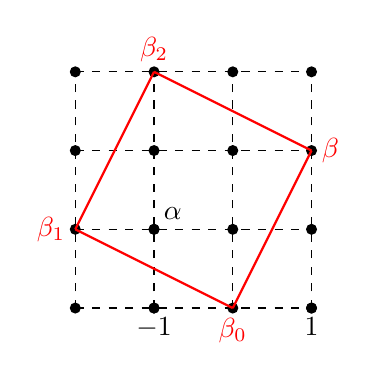
\begin{tikzpicture} 
\draw[dashed] (0,0) grid (3,3); 
\foreach \i in {0,...,3}     
\foreach \j in {0,...,3}         
\fill (\i,\j) circle (2pt);  
\draw[red,thick] 
(2,0)--(0,1) node[anchor=east] {$\beta_1$} 
(0,1)--(1,3) node[anchor=south] {$\beta_2$} 
(1,3)--(3,2) node[anchor=west] {$\beta$} 
(3,2)--(2,0) node[anchor=north] {$\beta_0$} ;
\fill (1,1) circle (2pt) node[anchor=south west] {$\alpha$}  ;
\fill (1,0) circle (2pt) node[anchor=north] {$-1$}  ;
\fill (3,0) circle (2pt) node[anchor=north] {$1$}  ;
\end{tikzpicture}
\caption{Division algorithm in $\Z[i]$.}
\label{fig:Z[i]}
\end{figure}

We know that $\Z$ and $\R[X]$ are both principal. The proofs 
are very similar, as both use the division algorithm essentially in the same way. 
The following result takes advantage of this fact. 

\begin{proposition}
	Let $R$ be an euclidean domain. Then $R$ is principal.	
\end{proposition}

\begin{proof}
	Let $I$ be an ideal of $R$. If $I=\{0\}$, then $I=(0)$ and hence 
	it is principal. So we may
	assume that $I\ne\{0\}$. Let $y\in I\setminus\{0\}$ be such that
	$\varphi(y)$ is minimal. We claim that $I=(y)$. 
	If $z\in I$, then $z=yq+r$, where $r=0$ or $\varphi(r)<\varphi(y)$. 
	The minimality of $\varphi(y)$ implies that $r=0$. Thus $z=yq\in (y)$ and 
	it follows that 
	$I=(y)$. 
\end{proof}

\begin{example}\
	Since $\Z[i]$ is euclidean, then it is principal.
\end{example}
 
\begin{example}
	The rings $\Z[\sqrt{-5}]$ and $\Z\left[\sqrt{-3}\right]$ are
	not principal. Why?
\end{example}

The ring $\Z[\frac{1+\sqrt{-19}}{2}]$ is an 
example of a ring that is principal and not euclidean. We will not prove this
fact in these notes. For a proof 
for example see \cite{MR967349}, \cite{MR3665445} or \cite{MR314831}.


\begin{definition}
	Let $R$ be an integral domain. Then $R$ is a 
	\textbf{unique factorization domain}
	if the following statements hold:
	\begin{enumerate}
	\item Each $x\in R\setminus\{0\}$ that is not a unit can be written as $x=c_1\cdots c_n$ for irreducibles $c_1,\dots,c_n$. 
	\item If $x=c_1\cdots c_n=d_1\cdots d_m$ for irreducibles $c_1,\dots,c_n$ and $d_1,\dots,d_m$, then $n=m$ and there exists $\sigma\in\Sym_n$ such that $c_i$ and $d_{\sigma(i)}$ are
		associate for all $i\in\{1,\dots,n\}$. 
	\end{enumerate}
\end{definition}

It is important to remark that some rings 
have factorizations and this factorization is not unique. 
In fact, if $N$ is a square-free integer, $\Z[\sqrt{N}]$ is noetherian and hence it   
has factorization. This fact will be proved in the proof of the following theorem. 
However, not all these rings with be euclidean domains. 

\begin{theorem}
	Let $R$ be a principal domain. 
	Then $R$ is a unique factorization domain.
\end{theorem}

\begin{proof}
	We divide the proof into three steps. 
	\begin{claim}
		$R$ is noetherian. 	
	\end{claim}
	
	This is trivial, as every ideal is, in particular, finitely-generated by assumption.   

	\begin{claim}
		$R$ admits factorizations. 	
	\end{claim}
	
	Let $x\in R\setminus\{0\}$ be such that $x\not\in\mathcal{U}(R)$. If $x$ is irreducible, 
	there is nothing to prove. If not, $x=x_1x_2$ with $x_1\not\in\mathcal{U}(R)$ and
	$x_2\not\in\mathcal{U}(R)$. If $x_1$ and $x_2$ are both irreducibles, 
	we are done. If not, say $x_1$ can be written as $x_1=x_{11}x_{12}$ with
	$x_{11}\not\in\mathcal{U}(R)$ and $x_{12}\not\in\mathcal{U}(R)$. If this process
	does not terminate, it means that there is a sequence of ideals
	\[
	(x)\subsetneq (x_1)\subsetneq (x_{11})\subsetneq\cdots 
	\]
	that does not stabilize, which contradicts the fact that $R$ is noetherian.  
	
	\begin{claim}
		$R$ admits unique factorization.	
	\end{claim}
	
	Let $x\in R$ be such that $x$ factorizes into irreducibles as 
	$x=c_1\cdots c_n=d_1\cdots d_m$. We may assume that $n\leq m$. We proceed by 
	induction on $m$. If $m=1$, then 
	$n=1$ and $c_1=d_1$. If $m>1$, then, since $c_1$ is prime and 
	$c_1\mid d_1\cdots d_m$, it follows that $c_1\mid d_j$ for some $j$, say $c_1\mid d_1$ (here is precisely where the permutation $\sigma$ appears). Since
	$d_1$ is irreducible, $c_1$ and $d_1$ are associate, that is
	$c_1=ud_1$ for some $u\in\mathcal{U}(R)$. Then
	\[
	c_1c_2\cdots c_n=(ud_1)c_2\cdots c_n=d_1d_2\cdots d_m. 
	\]
	Since $d_1\ne 0$,  
	\[
	d_1(uc_2\cdots c_n-d_2\cdots d_m)=0,
	\]
	which implies that $(uc_2)\cdots c_n=d_2\cdots d_m$ because $R$ is an integral domain. Note
	that $uc_2$ is irreducible and hence 
	the claim follows by the inductive hypothesis. 
\end{proof}

It is interesting to remark that the proof 
of the previous theorem is exactly the proof
one does for $\Z$. 

\begin{example}
	The ring $\Z[i]$ is a unique factorization domain. 	
\end{example}

We conclude the lecture with an example 
of a noetherian domain that is not a unique factorization domain. 

\begin{example}
	The ring $R=\Z[\sqrt{-6}]$ is not a unique factorization domain. In fact,
	\[
	10=2\cdot 5=(2+\sqrt{-6})(2-\sqrt{-6}).
	\]	
	Note that $N(a+b\sqrt{-6})=a^2+6b^2\ne 2$. This implies that $2$ is irreducible, as 
	if $2=\alpha\beta$, then $4=N(2)=N(\alpha)N(\beta)$. 
	Similarly, $5$ is irreducible. It is an exercise to prove that 
	$2+\sqrt{-6}$ and $2-\sqrt{-6}$ are both irreducible. 
\end{example}

\chapter{}

\begin{theorem}[Fermat]
\index{Fermat's theorem}
	Let $p\in\Z_{>0}$ be a prime number. The following statements are equivalent:
	\begin{enumerate}
	    \item $p=2$ or $p\equiv1\bmod 4$.
	    \item There exists $a\in\Z$ such that $a^2\equiv-1\bmod p$.
	    \item $p$ is not irreducible in $\Z[i]$.
	    \item $p=a^2+b^2$ for some $a,b\in\Z$.
	\end{enumerate}
\end{theorem}

\begin{proof}
    We first prove that $1)\implies 2)$. If $p=2$, take $a=1$. If $p=4k+1$ for some $k\in\Z$, then
    by Fermat's little theorem, the polynomial 
    $X^{p-1}-1\in(\Z/p)[X]$ has roots $1,2,\dots,p-1$. Write
    \[
    (X-1)(X-2)\cdots (X-(p-1))=X^{p-1}-1=X^{4k}-1=(X^{2k}+1)(X^{2k}-1)
    \]
    in $(\Z/p)[X]$. Since $p$ is prime, $\Z/p$ is a field and hence 
    $(\Z/p)[X]$ is a unique factorization domain (because it is euclidean). Thus 
    there exists $\alpha\in\Z/p$ such that $\alpha^{2k}+1=0$. To finish the proof
    take $a=\alpha^k$. 
    
    We now prove that $2)\implies 3)$. If $a^2\equiv-1\bmod p$, then $a^2+1=kp$ 
    for some $k\in\Z$. Since $(a-i)(a+i)=a^2+1=kp$, then $p$ divides $(a-i)(a+i)$. Let us prove that $p$ is not prime in $\Z[i]$. 
    We claim that $p$ does not divide $a-i$ in $\Z[i]$. Indeed, if $p\mid a-i$, then
    $a-i=p(e+fi)$ for some $e,f\in\Z$ and this implies that $1=pf$, a contradiction. Similarly,
    $p$ does not divide $a+i$. Thus $p$ is not prime in $\Z[i]$ 
    and hence it is not irreducible in $\Z[i]$ (because in $\Z[i]$ primes and irreducible coincide). 
    
    We now prove that $3)\implies 4)$. If $p=(a+bi)(c+di)$ with $a+bi\not\in\mathcal{U}(\Z[i])$
    and  $c+di\not\in\mathcal{U}(\Z[i])$, then
    \[
    p^2=N(p)=N(a+bi)N(c+di)=(a^2+b^2)(c^2+d^2)
    \]
    in $\Z$. Since $\Z$ has unique factorization, it follows that $p=a^2+b^2$. 
    
    Finally we prove that $4)\implies 1)$. 
    The only possible remainders after division by four are $0,1,2$ and $3$.  
    For all $a$, either $a^2\equiv 0\bmod 4$ or $a^2\equiv 1\bmod 4$. 
    If $p\equiv3\bmod 4$, then $p$ is never a sum of two squares, as 
    $a^2+b^2\equiv 0\bmod 4$, $a^2+b^2\equiv 1\bmod 4$ or $a^2+b^2\equiv 2\bmod 4$. 
\end{proof}

\begin{exercise}
\label{xca:Z[i]irreducibles}
Find the irreducible elements of $\Z[i]$. 
\end{exercise}


\topic{Zorn's lemma}

\begin{definition}
A non-empty set $R$ is said to be a \textbf{partially ordered set} (or poset, for short) 
if there is a subset $X\subseteq R\times R$ such that
\begin{enumerate}
    \item $(r,r)\in X$ for all $r\in R$, 
    \item if $(r,s)\in X$ and $(s,t)\in X$, then $(r,t)\in X$, and 
    \item if $(r,s)\in X$ and $(s,r)\in X$, then $r=s$. 
\end{enumerate}
\end{definition}

The set $X$ is a partial order relation on $R$.  
We will use the following notation: $(r,s)\in X$ if and only if $r\leq s$. Moreover, 
$r<s$ if and only if $r\leq s$ and $r\ne s$. 

\begin{definition}
Let $R$ be a poset and $r,s\in R$. Then $r$ and $s$ are \textbf{comparable}
if either $r<s$ or $s<r$.
\end{definition}

\begin{example}
    Let $U=\{1,2,3,4,5\}$ and $T$ be the set of subsets of $U$. Then $T$ is a poset
    with the usual inclusion, that is $C\leq D$ if and only if $C\subseteq D$. The subsets
    $\{1,2\}$ and $\{3,4\}$ of $U$ are elements of $T$ that are not comparable. 
\end{example}

\begin{definition}
    Let $R$ be a poset and $r\in R$. Then $r$ is \textbf{maximal} in $R$ if 
    $r\leq t$ implies $r=t$. 
\end{definition}

\begin{example}
    $\Z$ has no maximal elements. 
\end{example}

\begin{example}
Let $R=\{(x,y)\in\R^2:y\leq0\}$ with $(x_1,y_1)\leq(x_2,y_2)$ if and only if $x_1=x_2$ and $y_1\leq y_2$. Then
$R$ is a poset and each $(x,0)$ is maximal. Thus $R$ has infinitely many maximal elements.
\end{example}

\begin{definition}
    Let $R$ be a poset and $S$ be a non-empty subset of $R$. An \textbf{upper bound}
    for $S$ is an element $u\in R$ such that $s\leq u$ for all $s\in S$. 
\end{definition}

\begin{example}
    Let $S=\{6\Z,12\Z,24\Z\}$ be a subset of the set of subgroups of $\Z$ partially ordered by 
    the inclusion. Then 
    $6\Z=6\Z\cup 12\Z\cup 24\Z$ is an upper bound of the subset~$S$. 
\end{example}

\begin{definition}
    Let $R$ be a poset. A \textbf{chain} is a non-empty subset $S$ of $R$ such that
    any two elements of $S$ are comparable. 
\end{definition}

We now state Zorn's lemma:

\begin{quote}
\index{Zorn's lemma}
Let $R$ be a poset such that 
every chain in $R$ admits an upper bound in $R$. 
Then $R$ contains a maximal element. 
\end{quote}

It is not intuitive, but it is logically equivalent to a more 
intuitively statement in set theory, the Axiom of Choice, 
which says every Cartesian product of non-empty sets is non-empty. 
It is more an axiom than a lemma. 
The reason for calling Zorn’s lemma a lemma rather 
than an axiom is purely historical.

\begin{definition}
	\index{Ideal!maximal}
	Let $R$ be a ring. An ideal $I$ of $R$ is said to be \textbf{maximal}
	if $I\ne R$ and if $J$ is an ideal of $R$ such that $I\subseteq J$, then 
	either $I=J$ or $J=R$. 
\end{definition}

If $p$ is a prime number, then $p\Z$ is a maximal ideal of $\Z$.

\begin{exercise}
Let $R$ be a commutative ring. Prove that $R$ is a 
field if and only if $\{0\}$ is a maximal ideal of $R$. 	
\end{exercise}

\begin{exercise}
Let $R$ be a commutative ring and $I$ be an ideal of $R$. Prove that $I$ is maximal
if and only if $R/I$ is a field.  	
\end{exercise}

The following application of Zorn's lemma uses 
the identity of a ring. 

\begin{theorem}[Krull]
\index{Krull's theorem}
	Let $R$ be a ring. Each proper ideal $I$ of $R$ 
	is contained in a maximal ideal. 
	In particular, all rings have maximal ideals. 	
\end{theorem}

\begin{proof}
	Let $X=\{J:J\text{ is an ideal of $R$ such that }I\subseteq J\subsetneq R\}$.
	Since $I\in X$, it follows that $X$ is non-empty. Moreover, $X$ is a poset
	with respect to the inclusion. If $C$ is a chain in $X$ (say for example
	an increasing sequence
	\[
	I_1\subseteq I_2\subseteq\cdots
	\]
	of proper ideals of $R$ containing $I$), then 
	$\cup_{J\in C}J$ is an upper bound for $C$, as $\cup_{J\in C}J$ is an ideal and
	$\cup_{J\in C}J\ne R$ because $1\not\in\cup_{J\in C}J$. 	Zorn's lemma implies that
	there exists a maximal element $M\in X$. We claim that $M$ is a maximal ideal of $R$. The definition
	of $X$ implies that $M$ is a proper ideal of $R$ that contains $I$. If $M_1$ is a proper ideal of $R$
	such that $M\subseteq M_1$, it follows that $I\subseteq M_1$ and hence $M_1\in X$. The maximality
	of $M$ implies that $M=M_1$.  
\end{proof}

In the proof of previous theorem it is crucial to consider rings with 
identity. 

\begin{exercise}
	Compute the maximal ideals of $\R[X]$ and $\C[X]$. 	
\end{exercise}

One can also compute the maximal ideals of $K[X]$ for any field $K$. 

\begin{exercise}
	Let $R$ be a principal domain and $p\in R\setminus\{0\}$. Then $p$ is irreducible 
	if and only if $(p)$ is maximal.	
\end{exercise}

\begin{example}
	The ideal $(X^2+2X+2)$ is maximal in $\Q[X]$ because
	\[
	X^2+2X+2=(X+1)^2+1
	\]
	has degree two and no rational roots. 
	Hence $X^2+2X+2$ is irreducible in $\Q[X]$ and it generates 
	a maximal ideal. 	
\end{example}

% \begin{exercise}
% 	Let $R$ be a commutative ring and $I$ be an ideal of $R$. Then 
% 	$I$ is maximal if and only if $R/I$ is a field. 
% \end{exercise}

\begin{example}
	Let $R=(\Z/2)[X]$ and $f(X)=X^2+X+1$. Since $f(X)$ is irreducible (because $\deg f(X)=2$ and
	$f(X)$ has no roots in $\Z/2$, it follows that $(f(X))$ is a maximal ideal. 
	Thus $R/I$ is a field. 
\end{example}

\begin{exercise}
	Compute the maximal ideals of $\Z/n$. 	
\end{exercise}

\begin{exercise}
\label{xca:Jacobson}
\index{Jacobson's radical}
	Let $R$ be a commutative ring and $J(R)$ be the intersection of all maximal ideals 
	of $R$. Prove that $x\in J(R)$ 
	if and only if $1-xy\in\mathcal{U}(R)$ for all $y\in R$. The ideal $J(R)$ is proper
	and it is known
	as the \textbf{Jacobson's radical} of $R$.  	
\end{exercise}

We conclude the lecture with a different application of Zorn's lemma.  

\begin{exercise}
	Prove that every non-zero vector space has a basis.
\end{exercise}

The previous exercise can be used to solve the following exercises:

\begin{exercise}
\label{xca:extend}
    Every linearly independent subset of a non-zero vector space
    $V$ can be extended to a basis of $V$.
\end{exercise} 

Hint: If $X$ is a linearly independent set, a basis 
of $V$ that contains $X$ will be found as a maximal linearly independent set 
containing $X$. 

\begin{exercise}
    Let $V$ be a vector space. Prove that every subspace $U$ of $V$ is a direct summand of $V$, that is
    $V=U\oplus W$ for some subspace $W$ of $V$. 
\end{exercise}

\begin{exercise}
    Prove that every spanning set of a non-zero vector space
    contains a basis. 
\end{exercise}

\begin{exercise}
\label{xca:fx=cx}
    Prove that there exists a group homomorphism $f\colon\R\to\R$ that 
    is not of the form $f(x)=\lambda x$ for some $\lambda\in\R$. 
\end{exercise}


\begin{exercise}
\label{xca:Rn=R}
    Prove that the abelian groups $\R^n$ and $\R$ are isomorphic.
\end{exercise}

\begin{exercise}
\label{xca:aut}
    Prove that if $G$ is a group such that $|G|>2$, then $|\Aut(G)|>1$.
\end{exercise}

\topic{The characteristic of a ring}

\begin{definition}
Let $R$ be a ring. If there is a least positive integer $n$ such that 
$nx=0$ for all $x\in R$, then $R$ has \textbf{characteristic} $n$, i.e. $\ch R=n$. If no such $n$ exists, 
then $R$ is of characteristic zero. 
\end{definition}

Easy examples: $\ch\Z=0$ and $\ch\Z/n=n$.

\begin{proposition}
    Let $R$ be a ring such that $\ch R=n>0$,
    \begin{enumerate}
        \item The map $f\colon \Z\to R$, $m\mapsto m1$, is a ring homomorphism and $\ker f=n\Z$.  
        \item $n=\min\{k\in\Z_{>0}:k1=0\}$.
        \item If $R$ is a domain, then $n$ is a prime number.
    \end{enumerate}
\end{proposition}

\begin{proof}
    We leave 1) as an exercise. 
    
    Let us prove 2). Let $n_1=\min\{k\in\Z_{>0}:k1=0\}$. Clearly 
    $n\geq n_1$. For $x\in R$,
    $n_1x=n_1(1x)=(n_11)x=0x=0$ 
    and hence $n_1\geq n$. 
    
    Finally we prove 3). If $n$ is not prime, say
    $n=rs$ with $1<r,s<n$. Then 
    \[
    0=n1=(rs)1=(r1)(s1)
    \]
    and hence $r1=0$ or $s1=0$, a contradiction. 
\end{proof}

\begin{exercise}
\label{xca:freshman_dream}
\index{Freshman's dream}
    Let $R$ be a commutative ring of prime characteristic $p$. 
    \begin{enumerate}
        \item If $x,y\in R$, then $(x+y)^{p^n}=x^{p^n}+y^{p^n}$ for all $n\geq0$. 
        \item The map $R\to R$, $x\mapsto x^{p^n}$, is a ring homomorphism for all $n\geq0$.
    \end{enumerate}
\end{exercise}

Hint: Use induction on $n$ and the fact that the prime number $p$ divides 
$\binom{p}{k}$ for all $k\in\{1,2,\dots,p-1\}$. Alternatively, one could use
that the prime number $p$ divides $\binom{p^n}{k}$ for all 
$k\in\{1,2,\dots,p^n-1\}$. 


\topic{Group algebras}

We now discuss an important family of examples. 
Fix a field $K$. 
For a finite group $G$ let $K[G]$ be the vector space (over $K$)
with basis $\{g:g\in G\}$. Then $K[G]$ is a ring
with
\[
\left(\sum_{g\in G}\lambda_gg\right)\left(\sum_{h\in G}\mu_hh\right)
=\sum_{g,h\in G}\lambda_g\mu_h(gh).
\] 

Thus $K[G]$ is a ring and also a vector space (over $K$) and these structures
are somewhat compatible. Note that
\[
(\lambda a+\mu b)c=\lambda (ac)+\mu (bc),\quad
a(\lambda b+\mu c)=\lambda (ab)+\mu (ac)
\]
for all $\lambda,\mu\in K$ and $a,b,c\in K[G]$. 

\begin{definition}
\index{Algebra}
Let $A$ be a ring. Then $A$ is an algebra (over the field $K$) if $A$ is a vector space (over $K$)
such that $\lambda(ab)=(\lambda a)b=a(\lambda b)$ for all $\lambda\in K$ and $a,b\in A$. 
\end{definition}

Other examples of algebras are 
polynomial rings $K[X]$ and $K[X,Y]$ and matrix rings $M_n(K)$.  

\begin{example}
	If $A$ is an algebra, then $M_n(A)$ is an algebra.	
\end{example}

The ring $K[G]$ is commutative if and only if $G$ is abelian. Moreover,
$K[G]$ is a vector space of dimension $\dim K[G]=|G|$.

\begin{example}
	Let $G=\langle g:g^3=1\rangle=\{1,g,g^2\}\simeq C_3$ be the cyclic group of order three. 
	If $\alpha=a_11+_2g+a_3g^2$ and $\beta=b_11+b_2g+b_3g^2$, then
	\[
		\alpha\beta=(a_1b_1+a_2b_3+a_3b_2)1+(a_1b_2+a_2b_1+a_3b_3)g+a_1b_3+a_2b_2+a_3b_1)g^2.
	\]
	One can check that $\C[G]\simeq\C[X]/(X^3-1)$. 
\end{example}

In general, one proves that the group algebra of $C_n$, the cyclic group of order $n\geq2$, 
is isomorphic to $\C[X]/(X^n-1)$.

\begin{exercise}
\label{xca:RC3}
	Prove that $\R[C_3]\simeq\R\times\C$. 	
\end{exercise}

\begin{exercise}
	Let $G=\{1,g\}\simeq C_2$ be the cyclic group of order two. The product
	of $\C[G]$ is 
	\[
	(a1+bg)(c1+gd)=(ac+bd)1+(ad+bc)g.
	\]
	Prove that the map $\C[G]\to \C\times \C$, $a1+bg\mapsto (a+b,a-b)$, 
	is a linear isomorphism of rings. 
\end{exercise}

\begin{exercise}
	Let $K=\Z/2$ and $G=\{1,g\}\simeq C_2$ be the cyclic group of order two. 
	Prove that the map $K[G]\to\begin{pmatrix}
		K&K\\
		0&K
	\end{pmatrix}$, $a1+bg\mapsto\begin{pmatrix}
		a+b&b\\
		0&a+b		
	\end{pmatrix}$, is a linear isomorphism of rings.
\end{exercise}

The group ring has the following property, which is left as an exercise. 
Let $A$ be an algebra and
$G$ be a finite group. If $f\colon G\to\mathcal{U}(A)$ is a group homomorphism, 
then there exists a unique algebra homomorphism $\varphi\colon K[G]\to A$ such that
$\varphi|_G=f$. 

\begin{example}
	Let $\D_3=\langle r,s:r^3=s^2=1,\,srs^{-1}=r^{-1}\rangle$ be the dihedral
	group of six elements. We claim that 
	\[
	\C[\D_3]\simeq\C\times\C\times M_2(\C).
	\]
	Let $\omega$ be a primitive root of one. Let 
	\[
	R=\begin{pmatrix}
		\omega&0\\
		0&\omega^2	
	\end{pmatrix},
	\quad
	S=\begin{pmatrix}
		0&1\\
		1&0
	\end{pmatrix}.
 	\]
 	One easily checks that $SRS^{-1}=R^{-1}$ and $R^3=S^2=\begin{pmatrix}
		1&0\\
		0&1	
	\end{pmatrix}$. It follows that there exists a group homomorphism
	$G\to\C\times\C\times M_2(\C)$ such that
	$r\mapsto (1,1,R)$ and $s\mapsto (1,-1,S)$. This group homomorphism
	is a ring isomorphism.  
\end{example}




 
\section{}

We will dedicate three lectures to the development of the character theory for complex representations 
of finite groups. Our approach will remain entirely elementary, 
relying solely on fundamental linear algebra principles over complex numbers.

\subsection{Group representations}

\begin{definition}
	\index{Representation}
	A \textbf{representation} (over the field $K$) of a group $G$ is a group homomorphism
	$\rho\colon G\to\GL(V)$, $g\mapsto\rho_g$, for some non-zero finite-dimensional 
        vector space $V$ (over $K$).
\end{definition}

\index{Representation!degree}
The \textbf{degree} of the representation $\rho\colon G\to\GL(V)$ will be the dimension of $V$. Note that
since $V$ is finite-dimensional, say $\dim V=n$, after fixing a basis of $V$ we get a \textbf{matrix representation} 
$\rho\colon G\to\GL(V)\simeq\GL_n(K)$ of $G$. Depending on the context, we will use either representations on vector spaces or matrix representations.  

\begin{example}
	We use group representations to show that 
	$G=\langle x,y:x^2=y^2=1\rangle$ is infinite. Note that
	\[
	\rho\colon G\to\GL_2(\C),
	\quad
	x\mapsto\begin{pmatrix}
		1&0\\
		0&-1	
	\end{pmatrix},\quad
 	y\mapsto\begin{pmatrix}
		1&1\\
		0&-1	
	\end{pmatrix},
 	\]
 	is a group homomorphism, as 
 	$\rho_x^2=\rho_y^2=\begin{pmatrix}
		1&0\\
		0&1	
	\end{pmatrix}$. We claim that the elements of the form $(xy)^n$ are
	different for all $n$. It is enough to show that   
	$(xy)^n=(xy)^m$, then $n=m$. Note that
	\[
	\rho_{xy}=\rho_x\rho_y=\begin{pmatrix}
		1&0\\
		0&-1	
	\end{pmatrix}
	\begin{pmatrix}
		1&1\\
		0&-1	
	\end{pmatrix}
	=\begin{pmatrix}
		1&1\\
		0&1	
	\end{pmatrix}.
	\]
	Thus $\rho_{xy}^n=\begin{pmatrix}
		1&n\\
		0&1	
	\end{pmatrix}$ and 
	$\rho_{xy}^m=\begin{pmatrix}
		1&m\\
		0&1	
	\end{pmatrix}$. Then 
	\[
	(xy)^n=(xy)^m\implies\rho_{xy}^n=\rho_{xy}^m\implies n=m.
	\] 
\end{example}

The previous example shows the power of group representations, even for infinite groups.   
However, in this course, we will work with complex finite-dimensional 
representations of finite
groups.  

\begin{example}
\index{Representation!trivial}
	If $G$ is a group, then $\rho\colon G\to\GL_1(\C)=\C^\times$, $g\mapsto 1$, 
	is a representation. This representation is known as the \textbf{trivial (complex) representation} of $G$. 	
\end{example}

\begin{example}
	The sign yields a representation of $\Sym_n$. It is the group homomorphism
	$\Sym_n\to\C^\times$, $\sigma\mapsto\sgn(\sigma)$.  	
\end{example}

\begin{example}
	Let $G=\langle g:g^6=1\rangle$ be the cyclic group of order six. Then
	\[
	\rho\colon G\to\GL_2(\C),
	\quad 
	g\mapsto\begin{pmatrix}1&1\\-1&0\end{pmatrix}
	\] 
	is a group representation of degree two. 
\end{example}

%To prove the following result we need
%the \emph{minimal polynomial characterization of diagonazability",  
%see for example, \cite[Corollary 2.5.12]{zbMATH06049469}.
%
%\begin{proposition}
%    Let $G$ be a finite group and $\rho\colon G\to\GL_n(\C)$ 
%    be a representation. Then
%    each $\rho_g$ is diagonalizable.
%\end{proposition}
%
%\begin{proof}
%    Since $g$ is finite, $g^m=1$ for some $m\in\Z_{>0}$. This means that $\rho_g$ is a root of $X^m-1\in\C[X]$. Since
%    the roots of the polynomial $X^m-1$ are all different and $X^m-1$ factorizes linearly on $\C[X]$, it follows
%    that the minimal polynomial of $\rho_g$ also factorizes linearly in $\C[X]$. Hence $\rho_g$ is diagonalizable.
%\end{proof}
%
%In page \pageref{rho_diagonalizable} we will see an alternative  
%proof of the previous proposition. 
%
\begin{definition}
	\index{Invariant!map}
    Let $\rho\colon G\to\GL(V)$ and $\psi\colon G\to\GL(W)$ be
    representations. A linear map $T\colon V\to W$ is said to be \textbf{invariant} 
    if the diagram
    \[\begin{tikzcd}
	V & V \\
	W & W
	\arrow["{\rho_g}", from=1-1, to=1-2]
	\arrow["T"', from=1-1, to=2-1]
	\arrow["{\psi_g}"', from=2-1, to=2-2]
	\arrow["T", from=1-2, to=2-2]
\end{tikzcd}
\]
    commutes for all $g\in G$, this means that 
    $\psi_gT=T\rho_g$ for all $g\in G$.
\end{definition}

It is convenient to introduce an alternative
notation for group representations. 
Let 
\[ 
\rho\colon G\to\GL(V),\quad g\mapsto \rho_g,
\]
be a representation. For
$g\in G$ and $v\in V$ write $g\cdot v=\rho_g(v)$. Then the following properties hold: 
\begin{enumerate}
	\item $1\cdot v=v$ for all $v\in V$, 
	\item $g\cdot (h\cdot v)=(gh)\cdot v$ for all $g,h\in G$ and $v\in V$, 
	\item $g\cdot (v+w)=g\cdot v+g\cdot w$ for all $g\in G$ and $v,w\in V$, and 
	\item $g\cdot (\lambda v)=\lambda (g\cdot v)$ for all $g\in G$, $\lambda\in\C$ and $v\in V$.  	
\end{enumerate}
Using this notation for the representations $\rho\colon G\to\GL(V)$ 
and $\psi\colon G\to\GL(W)$, a linear
map $T\colon V\to W$ is invariant if and only if
\[
T(g\cdot v)=g\cdot T(v)
\]
for all $v\in V$ and $g\in G$. 
Although we use the same notation for different representations, there is no risk of confusion. 

\begin{definition}
	\index{Representations!equivalence}
    The representations $\rho\colon G\to\GL(V)$ and $\psi\colon G\to\GL(W)$ are \textbf{equivalent}
    if there exists a bijective map $T\colon V\to W$ invariant with respect to $\rho$ and $\psi$.
\end{definition}

If the representations $\rho$ and 
$\psi$ are equivalent, we write 
$\rho\simeq\psi$. 

Now we can understand why we can alternatively use
representations or matrix representations. 

\begin{example}
\label{xca:change_of_basis}
Let $\rho\colon G\to\GL(V)$ be a representation, say, of degree 
$n=\dim V$. Choose a basis 
$B=\{v_1,\dots,v_n\}$ of $V$ and let 
\[
T\colon V\to\C^n,
\quad
\sum_{i=1}^n\lambda_iv_i\mapsto (\lambda_1,\dots,\lambda_n)
\]
the isomorphism that takes coordinates 
for the basis $B$. For each $g\in G$, 
the composition of linear maps 
\[
\C^n\xrightarrow[]{T^{-1}}V\xrightarrow[]{\rho_g} V
\xrightarrow[]{T}\C^n
\]
produces a representation 
$\psi\colon G\to\GL(C^n)$
%\quad 
%g\mapsto T\rho T^{-1},
%\]
is a representation 
of $G$ equivalent to $\rho$.   
\end{example}

\begin{example}
    Let $G=\Z/n$. The representations
    \begin{align*}
    &\rho\colon G\to\GL_2(\C),\quad
    m\mapsto
    \begin{pmatrix}
        \cos(2\pi m/n) & -\sin(2\pi m/n)\\
        \sin(2\pi m/n) & \cos(2\pi m/n)
    \end{pmatrix},
    \shortintertext{and}
    &\psi\colon G\to\GL_2(\C),\quad
    m\mapsto
    \begin{pmatrix}
        e^{2\pi im/n} & 0\\
        0 & e^{-2\pi im/n}
    \end{pmatrix},
    \end{align*}
    are equivalent, as $\rho_mT=T\psi_m$ for all $m\in G$ if $T=\begin{pmatrix}
        i&-i\\
        1&1
    \end{pmatrix}$.
\end{example}

\begin{definition}
	\index{Invariant!subspace}
    Let $\rho\colon G\to\GL(V)$
    a representation. A subspace $W$ of $V$ is said to be \textbf{invariant} (with respect to $\rho$)
    if $\rho_g(W)\subseteq W$ for all $g\in G$.
\end{definition}

Let $\rho\colon G\to\GL(V)$ be a representation. Then $\{0\}$ and $V$ are always   
invariant subspaces of~$V$. Moreover, if $W\subseteq V$ is invariant, then
the map $\rho|_W\colon G\to\GL(W)$, $g\mapsto (\rho_g)|_W$, is a representation. The
map $\rho|_W$ is the \textbf{restriction} of $\rho$ to $W$. 

\begin{example}
	If $\rho\colon G\to\GL(V)$ and $\psi\colon G\to\GL(W)$ are representations of a given group $G$ 
	and 
 $T\colon V\to W$
 is an invariant map, then the \textbf{kernel} 
	\[
	\ker T=\{v\in V:T(v)=0\}
	\]
	is an invariant of $V$ and the \textbf{image} 
	\[
		T(V)=\{T(v):v\in V\}
	\]
	is an invariant subspace of $W$. 
\end{example}


\begin{definition}
\index{Subrepresentation}
    Let $\rho\colon G\to\GL(V)$
    a representation. A \textbf{subrepresentation} of $\rho$ is a restricted representation 
    of the form $\rho|_W\colon G\to\GL(W)$ for some invariant subspace $W$ of $V$.
\end{definition}

%\begin{example}
%    Let $G=\langle g:g^3=1\rangle$ be the
%    cyclic group of order three
%    and
%    \[
%    \rho\colon G\to\GL_3(\R),
%    \quad
%    g\mapsto\begin{pmatrix}
%        0&1&0\\
%        0&0&1\\
%        1&0&0
%    \end{pmatrix}.
%    \]
%    The subspace
%    \[
%    W=\left\{
%    \begin{pmatrix}
%    x\\
%    y\\
%    z
%    \end{pmatrix}\in\R^3:x+y+z=0\right\}
%    \]
%    is a invariant subspace of $\R^3$.
%\end{example}

\begin{definition}
    \index{Representation!irreducible}
    A representation $\rho\colon G\to\GL(V)$ is \textbf{irreducible} if
    $\{0\}$ and $V$ are the only invariant subspaces of $V$.
\end{definition}

Degree-one representations are irreducible. 

The irreducibility 
of a representation, of course, depends on the base field. 
In the following example, it is crucial using real representations.

\begin{example}
    Let $G=\langle g:g^3=1\rangle$ be the
    cyclic group of order three
    and
    \[
    \rho\colon G\to\GL_3(\R),
    \quad
    g\mapsto\begin{pmatrix}
        0&1&0\\
        0&0&1\\
        1&0&0
    \end{pmatrix}.
    \]
    Note that in this example we work with a real representation! 
    It is a routine calculation to prove that 
    \[
    W=\left\{
    \begin{pmatrix}
    x\\
    y\\
    z
    \end{pmatrix}\in\R^3:x+y+z=0\right\}
    \]
    is an invariant subspace of $\R^3$. We claim that $W$ 
    is irreducible. Let $S$ be a non-zero invariant subspace of 
    $W$ and let $s=\begin{pmatrix}x_0\\y_0\\z_0\end{pmatrix}\in S$ be a non-zero element. Then
    \[
    t=\begin{pmatrix}y_0\\z_0\\x_0\end{pmatrix}
    =\begin{pmatrix}
        0&1&0\\
        0&0&1\\
        1&0&0
    \end{pmatrix}
    \begin{pmatrix}x_0\\y_0\\z_0\end{pmatrix}\in S.
    \]
    We claim that $\{s,t\}$ are linearly independent. If not, there exists $\lambda\in\R$ such that
    $\lambda s=t$. Thus $\lambda x_0=y_0$, $\lambda y_0=z_0$ and $\lambda z_0=x_0$. This implies that
    $\lambda^3x_0=x_0$. Since $x_0\ne 0$ (because if $x_0=0$, then $y_0=z_0=0$, a contradiction), it follows that
    $\lambda=1$ and hence $x_0=y_0=z_0$, a contradiction because $x_0+y_0+z_0=0$.
    Therefore $\dim S=2$ and hence $S=W$.
\end{example}

What happens in the previous example if we work over complex numbers?

\begin{exercise}
    Let $\rho\colon G\to\GL(V)$ be a degree-two representation. Prove that
    $\rho$ is irreducible if and only if there is no common eigenvector for the $\rho_g$, $g\in G$.
\end{exercise}

The previous exercise can be used to show that the representation
$\Sym_3\to\GL_2(\C)$
of the symmetric group $\Sym_3$
given by
\[
(12)\mapsto\begin{pmatrix}
-1&-1\\0&1
\end{pmatrix},
\quad
(123)\mapsto\begin{pmatrix}
-1&-1\\
1&0
\end{pmatrix},
\]
is irreducible.

\begin{example}
Let $\rho\colon G\to\GL_n(\C)$ and $\psi\colon G\to\GL_m(\C)$ be representations. One defines
the \textbf{direct sum} $\rho\oplus\psi$ of $\rho$ and $\psi$ as 
\[
\rho\oplus\psi\colon G\to\GL_{n+m}(\C),\quad
g\mapsto 
\begin{pmatrix}
\rho_g & 0\\
0 & \psi_g	
\end{pmatrix}.
\]
\end{example}

Let us describe the previous example without using matrix representations. If $V$ and 
$W$ are complex vector spaces, the (external) direct sum of $V$ and $W$ is defined
as the set $V\times W$ with the complex vector space structure given by
\[
(v,w)+(v_1,w_1)=(v+v_1,w+w_1),\quad
\lambda (v,w)=(\lambda v,\lambda w)
\]
for all $v,v_1\in V$, $w,w_1\in W$ and $\lambda\in\C$. 
If $\rho\colon G\to\GL(V)$ and $\psi\colon G\to\GL(W)$ are representations, 
the \textbf{direct sum} $\rho\oplus\psi$ of $\rho$ and $\psi$ is then 
\[
\rho\oplus\psi\colon G\to\GL(V\oplus W),\quad
g\mapsto (\rho\oplus\psi)_g,
\]
where $(\rho\oplus\psi)_g\colon V\oplus W\to V\oplus W$, 
$(v,w)\mapsto (\rho_g(v),\psi_g(w))$. Note that both 
$V\simeq V\oplus\{0\}$ and $W\simeq \{0\}\oplus W$ are
invariant subspaces of $V\oplus W$. 

\begin{definition}
    \index{Representation!completely reducible}
    A representation $\rho\colon G\to\GL(V)$ is said to be 
    \textbf{completely reducible}
    if $\rho$ can be decomposed as
    $\rho=\rho_1\oplus\cdots\oplus \rho_n$ for some irreducible
    representations $\rho_1,\dots,\rho_n$ of $G$. 
\end{definition}

Note that if $\rho\colon G\to\GL(V)$ is completely reducible and 
$\rho=\rho_1\oplus\cdots\oplus \rho_n$ for some irreducible representations 
$\rho_i\colon G\to\GL(V_i)$, $i\in\{1,\dots,n\}$, then 
each $V_i$ is an invariant subspace of $V$ and $V=V_1\oplus \cdots V_n$. 
Moreover, on some basis of $V$, the matrix  
$\rho_g$ can be written as 
\[
\rho_g=\begin{pmatrix}
(\rho_1)_g &  \\
& (\rho_2)_g  \\
&&\ddots\\
&&&(\rho_n)_g	
\end{pmatrix}.
\]

\begin{definition}
\index{Representation!decomposable}
\index{Representation!indecomposable}
A representation
$\rho\colon G\to\GL(V)$ is \textbf{decomposable} if $V$ can be decomposed as $V=S\oplus T$
where $S$ and $T$ are non-zero invariant subspaces of $V$. 
\end{definition}

A representation is 
\textbf{indecomposable} if it is not decomposable. 

\begin{exercise}
\label{xca:equivalence}
	Let $\rho\colon G\to\GL(V)$ and $\psi\colon G\to\GL(W)$ be equivalent representations.
	Prove the following facts:
	\begin{enumerate}
		\item If $\rho$ is irreducible, then $\psi$ is irreducible.
		\item If $\rho$ is decomposable, then $\psi$ is decomposable.
		\item If $\rho$ is completely reducible, then $\psi$ is completely reducible. 
	\end{enumerate}	
\end{exercise}

Since we are considering finite-dimensional vector spaces, our vector spaces are
Hilbert spaces, so they have
an inner product $V\times V\to\C$, $(v,w)\mapsto\langle v,w\rangle$.

\begin{definition}
    \index{Representation!unitary}
    A representation $\rho\colon G\to\GL(V)$ is \textbf{unitary} if
    $\langle \rho_gv,\rho_gw\rangle=\langle v,w\rangle$ for all $g\in G$ and $v,w\in V$.
\end{definition}

\begin{example}
Let $G$ be a finite group and $V=\C[G]$. The \textbf{left regular representation}
of $G$ is the representation
\[
L\colon G\to\GL(V),
\quad
g\mapsto L_g,
\]
where $L_g(h)=gh$. With the inner product
\[
\left\langle\sum_{g\in G}\lambda_gg,\sum_{g\in G}\mu_gg\right\rangle=\sum_{g\in G}\lambda_g\overline{\mu_g}
\]
the representation $L$ is unitary. Prove it! 
\end{example}



If $V$ is a vector space and $W$ is a subspace of $V$, 
\[
W^\perp = \{v\in V:\langle v,w\rangle=0\text{ for all $w\in W$}\}.
\]
is called the 
\textbf{orthogonal complement} of $W$. The following result is extremely important: 

\begin{proposition}
\label{pro:irr_or_dec}
Let $\rho\colon G\to\GL(V)$ be a unitary representation. Then $\rho$ is either
irreducible or decomposable.
\end{proposition}

\begin{proof}
	If $\rho$ is not irreducible, there exists an invariant subspace $W$ of $V$ such that
	$\{0\}\subsetneq W\subsetneq V$. Can we find an invariant complement? Yes, and this is because 
        our representation is unitary.  
	Then $V=W\oplus W^{\perp}$ as complex vector spaces, where 
	$W^\perp\ne\{0\}$. So $\rho$ will be decomposable if we can prove that
	$W^\perp$ is an invariant subspace of $V$. 
	Let $v\in W^\perp$, $w\in W$ and $g\in G$. Then  
	\[
	\langle \rho_g(v),w\rangle=\langle v,\rho_g^{-1}(w)\rangle=0   
	\]
	since $\rho_g^{-1}(w)\in W$, as $W$ is an invariant subspace of $V$. This means that 
	$\rho_g(v)\in W^\perp$ and hence $V=W\oplus W^{\perp}$ is decomposable.  
\end{proof}

\begin{theorem}[Weyl's trick]
\index{Weyl's trick}
    Every representation $\rho\colon G\to\GL_n(\C)$ 
    of a finite group is unitary.
\end{theorem}

\begin{proof}
    Let $V=\C^n$ and 
    $V\times V\to\C$, $(v,w)\mapsto (v\mid w)$, be an\footnote{It does not matter which inner product we have chosen. 
    We use this particular notation for our inner product of $V$ because  
    with this inner product, we will 
    produce a new inner product (denoted by $(v,w)\mapsto \langle v, w\rangle$) that will turn $\rho$ 
    into a unitary representation.} inner
    product on $V$. 
   
    A straightforward calculation shows that
    \[
    \langle v,w\rangle=\sum_{g\in G}(\rho_gv\mid \rho_gw)
    \]
    is an inner product of $V$. For example, 
    \begin{align*}
    \langle v,w+w_1\rangle&=\sum_{g\in G}(v\mid w+w_1)\\
    &=\sum_{g\in G}\left((v\mid w)+(v\mid w_1)\right)\\
    &=\sum_{g\in G}(v\mid w)+\sum_{g\in G}(v\mid w_1)\\
    &=\langle v,w\rangle+\langle v,w_1\rangle 
    \end{align*}
    holds for all $v,w,w_1\in V$. 
    
    Since
    \begin{align*}
    \langle\rho_gv,\rho_gw\rangle&=\sum_{h\in G}(\rho_h\rho_gv\mid \rho_h\rho_gw)\\
    &=\sum_{h\in G}(\rho_{hg}v\mid\rho_{hg}w)=\sum_{x\in G}(\rho_xv\mid\rho_xw)=\langle v,w\rangle,
    \end{align*}
    the representation $\rho$ is unitary.
\end{proof}

\label{rho_diagonalizable}
Weyl's trick has several interesting consequences:  

\begin{corollary}
\label{cor:consequences}
	Let $\rho\colon G\to\GL(V)$ be a representation of a finite group $G$. 
 The following properties
	hold:
	\begin{enumerate}
		\item $\rho$ is equivalent to a unitary representation.
		\item $\rho$ is either irreducible or decomposable.
		\item Each $\rho_g$ is diagonalizable. 
	\end{enumerate}
\end{corollary}

\begin{proof}
	The first claim follows from Example \ref{xca:change_of_basis} and 
	Weyl's trick. The second claim, from 1) and
	Proposition \ref{pro:irr_or_dec}. Finally, 3) follows 
	from Weyl's trick immediately, as unitary matrices are diagonalizable.  
\end{proof}

\begin{exercise}
\label{xca:not_decomposable}
    If $G$ is an infinite group, it is no longer true that every non-zero representation
    is either irreducible or decomposable. Find an example.
\end{exercise}

For the previous exercise consider the representation $\Z\to\GL_2(\C)$, 
$1\mapsto\begin{pmatrix}1&1\\0&1\end{pmatrix}$. 
\chapter{}

Recall that, by convention, we only consider complex 
finite-dimensional representations of finite groups.

\begin{theorem}[Maschke]
\index{Maschke theorem}
    Every representation of a finite group is completely reducible.
\end{theorem}

\begin{proof}
    Let $G$ be a finite group and $\rho\colon G\to\GL(V)$ be a representation of $G$. We proceed
    by induction on $\dim V$.
    If $\dim V=1$, the result is trivial, as degree-one representations are irreducible. Assume that
    the result holds for representations of degree $\leq n$. Suppose that $\rho$ has degree $n+1$. 
    If $\rho$ is irreducible, we are done. If not, write $V=S\oplus T$, where $S$ and $T$
    are non-zero invariant subspaces of $V$. Since $\dim S<\dim V$ and $\dim T<\dim V$, it follows from
    the inductive hypothesis that
    both $S$ and $T$ are spaces of completely reducible representations. 
    Thus $\rho$ is completely reducible.
\end{proof}

\begin{example}
    Let $G=\Sym_3$ and $\rho\colon G\to\GL_3(\C)$ be the representation given by
    \[
    (12)\mapsto\begin{pmatrix}
    0&1&0\\
    1&0&0\\
    0&0&1
    \end{pmatrix},\quad
    (123)\mapsto\begin{pmatrix}
    0&0&1\\
    1&0&0\\
    0&1&0
    \end{pmatrix}
    \]
    Then $\rho_g$ is unitary for all $g\in G$ (because $\rho_{(12)}$ and $\rho_{(123)}$ are both
    unitary). Moreover,
    \[
    S=\left\langle \begin{pmatrix}
    1\\1\\1
    \end{pmatrix}
    \right\rangle,
    \quad
    T=S^{\perp}=\left\langle
    \begin{pmatrix}
    -1\\1\\0
    \end{pmatrix},
    \begin{pmatrix}
    0\\-1\\1
    \end{pmatrix}
    \right\rangle,
    \]
    are irreducible invariant subspaces of $V=\C^3$. A direct calculation shows that
    in the orthogonal basis $\left\{\begin{pmatrix}
    1\\1\\1
    \end{pmatrix},
    \begin{pmatrix}
    -1\\1\\0
    \end{pmatrix},
    \begin{pmatrix}
    0\\-1\\1
    \end{pmatrix}
    \right\}$
    the matrices $\rho_{(12)}$ and $\rho_{(123)}$ can be written as
    \[
    \rho_{(12)}=\begin{pmatrix}
        1&0&0\\
        0&-1&1\\
        0&0&1
    \end{pmatrix},
    \quad
    \rho_{(123)}=
    \begin{pmatrix}
        1&0&0\\
        0&0&-1\\
        0&1&-1
    \end{pmatrix}.
    \]
\end{example}

\begin{exercise}
Let $G$ be a finite group.
Prove that there is a bijection between degree-one representations of $G$ and
degree-one representations of $G/[G,G]$.
\end{exercise}

\begin{lemma}[Schur]
    Let $\rho\colon G\to\GL(V)$ and $\psi\colon G\to\GL(W)$ be irreducible representations. If 
    $T\colon V\to W$ is a non-zero invariant map, then $T$ is bijective.  
\end{lemma}

\begin{proof}
    Since $T$ is non-zero and $\ker T$ is an invariant subspace of $V$, it follows that $\ker T=\{0\}$, as $\rho$ is irreducible. Thus 
    $T$ is injective. Since $T(V)$ is a non-zero invariant subspace of $W$, it follows from the fact that $\psi$ is irreducible 
    that $T$ is surjective. Therefore $T$ 
    is bijective.  
\end{proof}

Two applications:

\begin{proposition}
    If $\rho\colon G\to\GL(V)$ is an irreducible representation and $T\colon V\to V$ is invariant, then 
    $T=\lambda\id$ for some $\lambda\in\C$. 
\end{proposition}

\begin{proof}
    Let $\lambda$ be an eigenvector of $T$. Then $T-\lambda\id$ is invariant and it is 
    not bijective. Thus $T-\lambda\id=0$ by Schur's lemma.
\end{proof}

\begin{proposition}
    Let $G$ be a finite abelian group. If $\rho\colon G\to\GL(V)$ is an irreducible representation, then
    $\dim V=1$. 
\end{proposition}

\begin{proof}
    Let $h\in G$. Note that since $G$ is abelian, $T=\rho_h$ is invariant:
    \[
    T\rho_g=\rho_h\rho_g=\rho_{hg}=\rho_{gh}=\rho_g\rho_h=\rho_gT.
    \]
    By Schur's lemma, there exists $\lambda_h\in\C$ such that $\rho_h=\lambda_h\id$. If $v\in V\setminus\{0\}$, 
    then $V=\langle v\rangle$, as $\rho$ is irreducible. 
\end{proof}

\topic{Characters}

This lecture is devoted to study character theory. We prove
the first Schur orthogonality relation and present 
several applications.

\begin{definition}
	\index{Character}
	Let $\rho\colon G\to\GL(V)$ be a representation. The \textbf{character} of $\rho$ 
	is the map $\chi_\rho\colon G\to\C$, $g\mapsto\trace\rho_g$. 	
\end{definition}

If a representation $\rho$ is irreducible, its character is said to be an 
\textbf{irreducible character}. The \textbf{degree} of a character is the degree of the affording
representation. 

\begin{proposition}
	Let $\rho\colon G\to\GL(V)$ be a representation, $\chi$ be its character and $g\in G$.
	The following statements hold:
	\begin{enumerate}
		\item $\chi(1)=\dim V$. 
		\item $\chi(g)=\chi(hgh^{-1})$ for all $h\in G$.
		\item $\chi(g)$ is the sum of $\chi(1)$ roots of one of order $|g|$. 
		\item $\chi(g^{-1})=\overline{\chi(g)}$. 
		\item $|\chi(g)|\leq\chi(1)$.  
	\end{enumerate} 
\end{proposition}

\begin{proof}
	The first statement is trivial. 	To prove 2) note that
	\[
	\chi(hgh^{-1})=\trace(\rho_{hgh^{-1}})=\trace(\rho_h\rho_g\rho_h^{-1})=\trace\rho_g=\chi(g).
	\]
	Statement 3) follows from the fact that the trace of $\rho_g$ is the sum
	of the eigenvalues of $\rho_g$ and these numbers are roots of the polynomial
	$X^{|g|}-1\in\C[X]$. To prove 4) write $\chi(g)=\lambda_1+\cdots+\lambda_k$, where 
	the $\lambda_j$ are roots of one. Then
	\[
	\overline{\chi(g)}=\sum^k_{j=1}\overline{\lambda_j}
	=\sum_{j=1}^k\lambda_j^{-1}
	=\trace(\rho_g^{-1})
	=\trace(\rho_{g^{-1}})
	=\chi(g^{-1}).
	\] 
	Finally, we prove 5). Use 3) to write $\chi(g)$ as the sum of
	$\chi(1)$ roots of one, say $\chi(g)=\lambda_1+\cdots+\lambda_k$ for
	$k=\chi(1)$. Then 
	\[
	|\chi(g)|=|\lambda_1+\cdots+\lambda_k|\leq |\lambda_1|+\cdots+|\lambda_k|
	=\underbrace{1+\cdots+1}_{\text{$k$-times}}=k.
	\]
\end{proof}

If two representations are equivalent, their characters are equal.

\begin{definition}
	Let $G$ be a group and 
	$f\colon G\to\C$ be a map. Then $f$ is a \textbf{class function} if
	$f(g)=f(hgh^{-1})$ for all $g,h\in G$. 	
\end{definition}

Characters are class functions. 

\begin{proposition}
    If $\rho\colon G\to\GL(V)$ and
    $\psi\colon G\to\GL(W)$ are representations, then
    $\chi_{\rho\oplus\psi}=\chi_\rho+\chi_\psi$.
\end{proposition}

\begin{proof}
  For $g\in G$, it follows that 
  $(\rho\oplus\psi)_g=
  \begin{pmatrix}
    \rho_g & 0\\ 
    0 & \psi_g
  \end{pmatrix}$. 
  Thus  
  \[
    \chi_{\rho\oplus\psi}(g)=\trace((\rho\oplus\phi)_g)=\trace(\rho_g)+\trace(\psi_g)=\chi_\rho(g)+\chi_\psi(g).\qedhere
  \]
\end{proof}

Let $V$ be a vector space with basis $\{v_1,\dots,v_k\}$ and 
$W$ be a vector space with basis $\{w_1,\dots,w_l\}$. A 
\textbf{tensor product} of $V$ and $W$ is a vector space $X$ with 
together with a bilinear map 
\[
V\times W\to X,
\quad
(v,w)\mapsto v\otimes w,
\]
such that $\{v_i\otimes w_j:1\leq i\leq k,\,1\leq j\leq l\}$ is a  
basis of $X$. The tensor product of $V$ and $W$ is unique up to isomorphism 
and it is denoted by $V\otimes W$. Note that
\[
\dim(V\otimes W)=(\dim V)(\dim W).
\]

\begin{definition}
	Let $\rho\colon G\to\GL(V)$ and $\psi\colon G\to\GL(W)$ be representations. The \textbf{tensor product} of $\rho$ and $\psi$ is the representation of $G$ given by 
	\begin{gather*}
	\rho\otimes\psi\colon G\to\GL(V\otimes W),
	\quad 
	g\mapsto (\rho\otimes\psi)_g,
	\shortintertext{where}
	(\rho\otimes\psi)_g(v\otimes w)=\rho_g(v)\otimes \psi_g(w)
	\end{gather*}
	for $v\in V$ and $w\in W$.  	
\end{definition}

A direct calculation shows that the tensor product of representations is indeed a representation. 

\begin{proposition}
  	If $\rho\colon G\to\GL(V)$ and
    $\psi\colon G\to\GL(W)$ are representations, then
    \[
    \chi_{\rho\otimes\psi}=\chi_\rho\chi_\psi.
    \]
\end{proposition}

\begin{proof}
	For each $g\in G$ the map $\rho_g$ is diagonalizable. Let $\{v_1,\dots,v_n\}$
	be a basis of eigenvectors of $\phi_g$ and let $\lambda_1,\dots,\lambda_n\in\C$ be such that
	$\rho_g(v_i)=\lambda_iv_i$ for all $i\in\{1,\dots,n\}$. Similarly, 
	let $\{w_1,\dots,w_m\}$ be a basis of 
	eigenvectors of $\psi_g$ and $\mu_1,\dots,\mu_m\in\C$ be such that $\psi_g(w_j)=\mu_jw_j$ for all $j\in\{1,\dots,m\}$. Each 
	$v_i\otimes w_j$ is eigenvector of $\phi\otimes\psi$ with eigenvalue 
	$\lambda_i\mu_j$, as  
	\[
		(\rho\otimes\psi)_g(v_i\otimes w_j)=\rho_gv_i\otimes \psi_gw_j=\lambda_iv_i\otimes \mu_jv_j=(\lambda_i\mu_j)v_i\otimes w_j.
	\]
	Thus  
	$\{v_i\otimes w_j:1\leq i\leq n,1\leq j\leq m\}$ is a basis of eigenvectors and the 
	$\lambda_i\mu_j$ are the eigenvalues of $(\phi\otimes\psi)_g$. It follows that 
	\[
	\chi_{\rho\otimes\psi}(g)
	=\sum_{i,j}\lambda_i\mu_j
	=\left(\sum_i\lambda_i\right)\left(\sum_j\mu_j\right)
	=\chi_\rho(g)\chi_\psi(g).\qedhere 
	\]
\end{proof}

For completeness we mention without proof that
it is also possible to define the dual $\rho^*\colon G\to\GL(V^*)$  
of a representation
$\rho\colon G\to\GL(V)$ by the formula
\[
(\rho^*_gf)(v)=f(\rho^{-1}_gv),\quad
g\in G,\,f\in V^*\text{ and }v\in V.
\]  
We claim that the character of the dual representation is then 
$\overline{\chi_\rho}$. Let $\{v_1,\dots,v_n\}$ be a basis of $V$
and $\lambda_1,\dots,\lambda_n\in\C$ be such that $\rho_gv_i=\lambda_iv_i$ for all $i\in\{1,\dots,n\}$. If $\{f_1,\dots,f_n\}$ is the dual basis of $\{v_1,\dots,v_n\}$, then 
\[
(\rho^*_gf_i)(v_j)=f_i(\rho_g^{-1}v_j)
=\overline{\lambda_j}f_i(v_j)
=\overline{\lambda_j}\delta_{ij}
\]
and the claim follows. 
%\begin{proposition}
%	
%\end{proposition}
%
%\begin{proof}
%	Let $g\in G$ and $\{v_1,\dots,v_n\}$
%	be a basis of eigenvectors of $\rho_g$. Let
%	$\lambda_1,\dots,\lambda_n\in\C$ be such that $\rho_g(v_i)=\lambda_iv_i$ for all
%	$i\in\{1,\dots,n\}$. Let $\{f_1,\dots,f_n\}$ be the dual basis of $\{v_1,\dots,v_n\}$.
%	Since $\rho_g$ is invertible, each eigenvector of $\rho_g$ is non-zero. 
%	Thus $\rho_g(v_i)=\lambda_iv_i$ implies that 
%	$\rho_{g^{-1}}v_i=\lambda_i^{-1}v_i=\overline{\lambda_i}v_i$... 
%%	Now 
%%	\[
%		(\rho_g f_i)(v_j)=f_i(g^{-1}v_j)=\overline{\lambda_j}f_i(v_j)=\overline{\lambda_j}\delta_{ij}.
%	\]
%	
%	  
%	
%	 We claim
%	that $\{f_1,\dots,f_n\}$ is a basis of eigenvectors...
%	with $\overline{\lambda_1},\dots,\overline{\lambda_n}$. En efecto, si $gv_j=\lambda_jv_j$, entonces
%	$g^{-1}v_j=\lambda_j^{-1}v_j=\overline{\lambda_j}v_j$ (observemos que como $\phi_g$ es inversible, los $\lambda_j$ son no nulos). Luego
%	\[
%		(gf_i)(v_j)=f_i(g^{-1}v_j)=\overline{\lambda_j}f_i(v_j)=\overline{\lambda_j}\delta_{ij}.
%	\]
%	En conclusión
%	\[
%		\chi_{V^*}(g)=\sum_{i=1}^n\overline{\lambda_i}=\overline{\chi_V(g)}.\qedhere
%	\]	
%\end{proof}

Let $\rho\colon G\to\GL(V)$ and $\psi\colon G\to\GL(W)$ be representations of a finite group
$G$. Since $V$ and $W$ are vector spaces, the set 
\[
\Hom(V,W)=\{T\colon V\to W:\text{$T$ is linear}\}
\]
is a vector space with 
\begin{align*}
&(\lambda T)(v)=\lambda T(v) && \text{for all $\lambda\in\C$ and all $v\in V$,}\\ 
&(T+T_1)(v)=T(v)+T_1(v) &&\text{for all $v\in V$.}
\end{align*}
We claim that the set $\Hom_G(V,W)$ of invariant maps
is a subspace of $\Hom(V,W)$. Indeed, the zero map is clearly invariant. If $T,T_1\in\Hom_G(V,W)$ 
and $\lambda\in\C$, then
\[
(T+\lambda T_1)(\rho_g v)
=T(\rho_gv)+\lambda T_1(\rho_gv)
=\psi_gT(v)+\lambda \psi_gT_1(v)
=\psi_g((T+\lambda T_1)(v))
\]
for all $v\in V$. 
 
\begin{proposition}
	Let $\rho\colon G\to\GL(V)$ and $\psi\colon G\to\GL(W)$ be representations
	and $T\colon V\to W$ be a linear map. Then
	\[
	T^{\#}=\frac{1}{|G|}\sum_{g\in G}\psi_{g^{-1}}T\rho_g\in\Hom_G(V,W).
	\]
	Moreover, the map $\Hom(V,W)\to\Hom_G(V,W)$, $T\mapsto T^{\#}$, is linear and surjective.  
\end{proposition}

\begin{proof}
  Let $h\in G$ and $v\in V$. Then 
  \begin{align*}
	T^{\#}\phi_h(v)
	&=\frac{1}{|G|}\sum_{g\in G}\psi_{g^{-1}}T\phi_g\phi_h(v)
	=\frac{1}{|G|}\sum_{g\in G}\psi_{g^{-1}}T\phi_{gh}(v)\\
	&=\frac{1}{|G|}\sum_{x\in G}\psi_{hx^{-1}}T\phi_x(v)
	=\frac{1}{|G|}\sum_{x\in G}\psi_h\psi_{x^{-1}}T\phi_x(v)
	=\psi_hT^{\#}(v).
      \end{align*}

	  If $T\in\Hom_{\C[G]}(V,V)$, then 
      \[
	T^{\#}(v)=\frac{1}{|G|}\sum_{g\in G}\psi_{g^{-1}}T\phi_g(v)
	=\frac{1}{|G|}\sum_{g\in G}\psi_{g^{-1}}\psi_gT(v)
	=T(v)
      \]
      for all $v\in V$.
\end{proof}

If $\phi\colon G\to\GL(V)$ and $\psi\colon
	G\to\GL(W)$ are non-equivalent irreducible representations and $T\colon
	V\to W$ is a linear map, then $T^{\#}=0$, as 
	$T^{\#}\in\Hom_{\C[G]}(V,W)=\{0\}$ by the previous proposition and Schur's lemma.

\begin{theorem}[Ergodic theorem]
  Let $\rho\colon G\to\GL(V)$ and $\psi\colon G\to\GL(W)$ be irreducible representations. 
  If $T\colon V\to W$ is linear, then 
  $T^{\#}=(\dim V)^{-1}\trace(T)\id$.
\end{theorem}

\begin{proof}
  The previous proposition and Schur's lemma imply that
  $T^{\#}=\lambda\id$ for some $\lambda\in\C$.
  We now compute the trace of $T^{\#}$. On the one hand, 
  \[
	\trace(T^{\#})=\trace(\lambda\id)=(\dim V)\lambda.
  \]
  On the other hand.  
  \[
	\trace(T^{\#})
	=\frac{1}{|G|}\sum_{g\in G}\trace(\rho_{g^{-1}}T\rho_g)
	=\frac{1}{|G|}\sum_{g\in G}\trace(T)
	=\trace(T),
  \]
  as $\trace(ABA^{-1})=\trace(B)$ for all $A$ and $B$. 
  Hence 
  \[
  \trace(T^{\#})=(\dim V)^{-1}\trace(T)\id.\qedhere 
  \]
\end{proof}

We now prove Schur's orthogonality relations. We need some preliminary material. First recall that 
the matrix $E_{ij}$ is given by 
\[
(E_{ij})_{kl}=\delta_{ik}\delta_{jl},
\qquad
\delta_{xy}=\begin{cases}
    1 & \text{if $x=y$},\\
    0 & \text{otherwise}.
\end{cases}
\]
If $\rho\colon G\to\GL(V)\simeq\GL_n(\C)$ is a representation, then
$\rho_g$ is the matrix $(\rho_{ij}(g))$ and hence the character of $\rho$ is given by
\[
\chi_\rho(g)=\sum_{i=1}^n\rho_{ii}(g).
\]

\begin{lemma}
Let $\rho\colon G\to\GL(V)$ and $\psi\colon G\to\GL(W)$ be irreducible representations. Then
$(E_{ik}^\#)_{lj}=\langle\rho_{ij},\psi_{kl}\rangle$.
\end{lemma}

\begin{proof}
  We compute
  \begin{align*}
      (E_{ki}^\#)_{lj} &= \frac{1}{|G|}\sum_{g\in G}(\psi_{g^{-1}}E_{ki}\rho_g)_{lj}\\
      &=\frac{1}{|G|}\sum_{g\in G}\sum_{p,q}\psi_{lq}(g^{-1})(E_{ki})_{qp}(\rho_{ij}(g))_{pj}\\
      &=\frac{1}{|G|}\sum_{g\in G}\psi_{lk}(g^{-1})\rho_{ij}(g)\\
      &=\frac{1}{|G|}\sum_{g\in G}\overline{\psi_{kl}(g)}\rho_{ij}(g)=\langle \rho_{ij},\psi_{kl}\rangle.\qedhere
  \end{align*}
\end{proof}

\begin{theorem}[Schur]
    Let $\rho\colon G\to\GL(V)$ and $\psi\colon G\to\GL(W)$ be irreducible representations. 
    Then the following statements hold:
    \begin{enumerate}
        \item $\langle\rho_{ij},\psi_{kl}\rangle=0$ if $\rho$ and $\psi$ are not equivalent.
        \item $\displaystyle{\langle\rho_{ij},\rho_{kl}\rangle=\frac{1}{\dim V}\delta_{ik}\delta_{jl}}$.
    \end{enumerate}
\end{theorem}

\begin{proof}
    Let us prove the first claim. Since 
    $\rho$ and $\psi$ 
    are not equivalent, it follows from Schur's lemma that $\Hom_G(V,W)=\{0\}$.
    Thus $E_{ki}^\#\in\Hom_G(V,W)=\{0\}$ by the Ergodic theorem. 
    
    To prove the second claim, we use the previous lemma:
    \[
    (E_{ki}^\#)_{lj}=\langle\rho_{ij},\psi_{kl}\rangle
    =\frac{1}{\dim V}(\trace E_{ki})\delta_{lj}
    =\frac{1}{\dim V}\delta_{ki}\delta_{lj}.\qedhere
    \]
\end{proof}

Now we can prove Schur's first orthogonality relation.

\begin{theorem}[Schur]
Let $\rho\colon G\to\GL(V)$ and $\psi\colon G\to\GL(W)$ be irreducible representations. Then
\[
\langle\chi_\rho,\chi_\psi\rangle=
\begin{cases}
1 & \text{if $\rho\simeq\psi$,}\\
0 & \text{otherwise.}
\end{cases}
\]
\end{theorem}

\begin{proof}
    Let $n=\dim V$ and $m=\dim W$. We compute
    \begin{align*}
        \langle\chi_\rho,\chi_\psi\rangle
        &=\frac{1}{|G|}\sum_{g\in G}\chi_\rho(g)\overline{\chi_\psi}(g)\\
        %&=\frac{1}{|G|}\sum_{g\in G}\sum_{i=1}^n\sum_{j=1}^m\rho_{ii}(g)\overline{\psi_{jj}(g)}\\
        &=\sum_{1=1}^n\sum_{j=1}^m\frac{1}{|G|}\rho_{ii}(g)\overline{\psi_{jj}(g)}
        =\sum_{1=1}^n\sum_{j=1}^m\frac{1}{|G|}\langle \rho_{ii},\psi_{jj}\rangle
        =\begin{cases}
            1 & \text{if $\rho\simeq\psi$,}\\
            0 & \text{otherwise.}
        \end{cases}\qedhere
    \end{align*}
\end{proof}

Schur's theorem has several important corollaries.

If $\rho\colon G\to\GL(V)$ is an irreducible representaion of degree $n$, then
\[
\{\sqrt{n}\rho_{ij}:1\leq i,j\leq n\}
\]
is an orthonormal set.

% \begin{corollary}
%     If $\rho\colon G\to\GL(V)$ is an irreducible representaion of degree $n$, then
%     $\{\sqrt{n}\rho_{ij}:1\leq i,j\leq n\}$ is an orthonormal set.
% \end{corollary}

\begin{corollary}
    A finite group has finitely many classes of irreducible representations. 
\end{corollary}

\begin{proof}
    Let $G$ be a finite group. 
    Every isomorphism class of representations of $G$ contains a unitary representation. Since $\dim L(G)=|G|$, 
    it follows that $G$ admits $\leq|G|$ equivalence classes of irreducible representations. Let
    $\rho_1,\dots\rho_r$ be the representatives of the isomorphism classes of the 
    irreducible representations of $G$. For each $k$ let $n_k=\deg\rho_k$. Since
    the $n_1^2+\cdots n_r^2$ maps $\sqrt{n_k}(\rho_k)_{ij}$, $1\leq k\leq r$, $1\leq i,j\leq n_k$,
    form an orthonormal set of $L(G)$, it follows that
    $r\leq n_1^2+\cdots n_r^2\leq|G|$.
\end{proof}

Let $G$ be a finite group. Since $G$ has only finitely many non-equivalent 
irreducible representation, we will often say
that 
\[
\rho_1,\dots,\rho_r
\]
are \emph{the} irreducible representations of $G$, where it is assumed that
the $\rho_i$ form a complete set of 
representatives of irreducible representations of $G$. For each $i$ we write
$\chi_i=\chi_{\rho_i}$. The set of irreducible characters will be denoted
by 
\[
\Irr(G)=\{\chi_1,\dots,\chi_r\}.
\]

% If $G$ is a finite group, let $K(G)$ be the number of conjugacy classes of $G$. 
% We want to know how many irreducible representations are there. For that purpose, 
% we need to study the space of class functions. 

Recall that $L(G)=\{f\colon G\to\C\}$ is a vector space with
\[
    (f+g)(x)=f(x)+g(x),
    \quad
    \lambda f)(x)=\lambda f(x),
    \quad 
    f,g\in L(G),\,\lambda\in\C,\,x\in G.
\]
Let $C(G)$ be the subspace of class functions. 
We claim that $\dim C(G)=K(G)$, the number of conjugacy classes of $G$. If $C$ is a conjugacy class, 
then 
\[
\delta_C\colon G\to\C,\quad
\delta_C(x)=\begin{cases}
    1 & \text{if $x\in C$,}\\
    0 & \text{otherwise.}
\end{cases}
\]
is a class function. Let us prove that the 
set $\{\delta_C:C\text{ is a conjugacy class of $G$}\}$ is a basis of $C(G)$.  It is a generating set
because each $f$ can be written as 
\[
f=\sum_{C}f(C)\delta_C.
\]
The $\delta_C$ are linearly independent because they are orthogonal: 
If $C$ and $D$ 
are conjugacy classes of $G$, then 
\[
\langle\delta_C,\delta_D\rangle=\frac{1}{|G|}\sum_{x\in G}\delta_C(x)\overline{\delta_D(x)}
=\begin{cases}
|C|/|G| & \text{if $C=D$},\\
0 & \text{otherwise}.
\end{cases}
\]

\begin{corollary}
    Let $G$ be a finite group. There are at most $K(G)$ equivalence classes of irreducible representations of $G$.
\end{corollary}

\begin{proof}
    Non-equivalent representations have different characters. 
    Irreducible characters 
    form an orthonormal set, thus they are linearly 
    independent. Since irreducible characters
    are class functions, it follows that there are at most $K(G)$ irreducible different characters.  
\end{proof}

Let $m\in\Z_{>0}$. If $V$ is a vector space, we 
write $mV=V\oplus\cdots\oplus V$ ($m$-times). Similarly,
if $\rho$ is a representation, 
we write $m\rho=\rho\oplus\cdots\oplus\rho$ ($m$-times). 


\begin{theorem}
    Let $\rho_1,\dots,\rho_r$ be the irreducible representations of a finite group $G$. If 
	$\rho=\sum_{i_1}^rm_j\rho_j$ where $m_1,\dots m_r\in\Z_{\geq0}$, then
    $m_j=\langle \rho_\rho,\rho_j\rangle$ for all $j\in\{1,\dots,r\}$. 
\end{theorem}

\begin{proof}
    Write $\chi_\rho=\sum_{j=1}^rm_j\chi_j$. Then
    \[
    \langle\chi_\rho,\chi_i\rangle=\sum_{j=1}^r\langle\chi_j,\chi_i\rangle=m_i
    \]
    for all $i\in\{1,\dots,r\}$.
\end{proof}

The theorem states that the decomposition of a representation $\rho$ into irreducibles 
is unique and that it is determined (up to equivalence) by its character.

\begin{corollary}
    A representation $\rho$ is irreducible if and only if $\langle\chi_\rho,\chi_\rho\rangle=1$.
\end{corollary}

\begin{proof}
    We first decompose $\rho$ as a sum of irreducibles, say $\rho=\sum_{j=1}^rm_j\rho_j$ with $m_1,\dots,m_r\geq0$. Then
    $\langle\chi_\rho,\chi_\rho\rangle=\sum_{j=1}^rm_j^2$. Now $\langle\chi_\rho,\chi_\rho\rangle=1$ if and only if
    there is exactly one $j$ such that $m_j=1$ and $m_i=0$ for all $i\ne j$.  
\end{proof}

% As an example, the representation of $\Sym_3$ given by

\begin{exercise}
    Let $\rho\colon H\to\GL(V)$ be an irreducible
    representation of $H$ and 
    $f\colon G\to H$ be a surjective group homomorphism. Prove that the composition $\rho\circ f\colon G\to\GL(V)$ is an irreducible representation. 
\end{exercise}

% is not irreducible. as $\chi($

\begin{theorem}
    Let $G$ be a finite group and $L$ be its regular representation. 
    Then $L=\sum_{j=1}^rn_j\rho_j$, where $n_j=\deg\rho_j$. 
\end{theorem}

\begin{proof}
    Let $G=\{g_1,\dots,g_n\}$, $n=|G|$. If $g\in G$, since
    $L_g(g_i)=gg_i$ for all $i$, 
    the matrix of $L_g$ in the basis $\{g_1,\dots,g_n\}$ is then
    \begin{gather*}
    (L_g)_{ij}=\begin{cases}
        1 & \text{if $g_i=gg_j$},\\
        0 & \text{otherwise}.
    \end{cases}
    \shortintertext{Then}
    \chi_L(g)=\trace(L_g)=\sum_{i=1}^r(L_g)_{ii}=\begin{cases}
        |G| & \text{if $g=1$},\\
        0 & \text{otherwise}.
    \end{cases}
    \end{gather*}
    In particular, 
    \[
    \langle\chi_L,\chi_i\rangle=\frac{1}{|G|}\sum_{g\in G}\chi_L(g)\overline{\chi_i(g)}
    =\frac{1}{|G|}|G|\overline{\chi_i(1)}=n_i
    \]
    for all $i\in\{1,\dots,n\}$. 
\end{proof}

Now several corollaries. 

\begin{corollary}
    Let $G$ be a finite group and $\rho_1,\dots,\rho_r$ be the irreducible representations of $G$. 
    For each $k$ let $n_k=\deg\rho_k$. The following statements hold:
    \begin{enumerate}
        \item $|G|=n_1^2+\cdots+n_r^2$.
        \item $\{\sqrt{n_k}(\rho_k)_{ij}:1\leq k\leq r,\,1\leq i,j\leq n_k\}$
            is an orthonormal basis of $L(G)$. 
        \item $r$ is equal to the number of conjugacy classes of $G$. 
    \end{enumerate}
\end{corollary}

\begin{proof}
    Since $\chi_L=\sum_{j=1}^rn_j\chi_j$, the first claim follows. 
    The second claim follows from the orthogonality relations. Let us prove the third claim. Let $f\in C(G)$ and write $f$ 
    as a linear combination of the $(\rho_k)_{ij}$, say
    \[
    f=\sum_{i,j,k}\lambda_{ijk}(\rho_k)_{ij},\quad\lambda_{ijk}\in\C.
    \]
    If $x\in G$, then 
    \begin{align*}
    f(x)&=\frac{1}{|G|}\sum_{g\in G}f(g^{-1}xg)\\
    &=\frac{1}{|G|}\sum_{g\in G}\sum_{i,j,k}\lambda_{ijk}(\rho_k)_{ij}(g^{-1}xg)
    =\sum_{i,j,k}\lambda_{ijk} \frac{1}{|G|}\sum_{g\in G}(\rho_k)_{ij}(g^{-1}xg). 
    \end{align*}
    Let $T=(\rho_k)_x\colon V\to V$. Then
    \[
    T^{\#}=\frac{1}{|G|}\sum_{g\in G}(\rho_k)_{g^{-1}}(\rho_k)_x(\rho_k)_g
    =\frac{1}{|G|}\sum_{g\in G}(\rho_k)(g^{-1}xg)
    =\frac{1}{\dim V}\chi_k(x)\id
    \]
    by the Ergodic theorem and because 
    $\rho_k$ is a group homomorphism. Thus 
    \[
    f(x)=\sum_{i,j,k}\lambda_{ijk} \left((\rho_k)_x\right)_{ij}
    =\sum_{i,j,k}\lambda_{ijk}\frac{1}{\dim V}\chi_k(x)\delta_{ij}
    =\sum_{i,k}\lambda_{ijk}\frac{1}{n_k}\chi_k(x).\qedhere 
    \]
    This implies that $\dim C(G)\leq r$ and the claim follows. 
\end{proof}

In the following exercise, the reader is asked to provide a proof of the second 
Schur's orthogonality relation. 

\begin{exercise}
    Let $G$ be a finite group and 
    $C$ and $D$ be conjugacy classes of $G$. If $g\in C$ and $h\in D$, then
    \[
    \sum_{\chi\in\Irr(G)}\chi(g)\overline{\chi(h)}=
    \begin{cases}
    |G|/|C| & \text{if $C=D$},\\
    0 & \text{otherwise}.
    \end{cases}
    \]
\end{exercise}

\section{Lecture -- Week 8}
\label{8}

\subsection{Proof of the orthogonality relations}
\label{subsection:Schur_proof}

Let $G$ be a finite $\rho\colon G\to\GL(V)$ and $\psi\colon G\to\GL(W)$ be representations. We know that
these representations are equivalent to matrix representations, say 
$\rho\colon G\to\GL_n(\C)$
and $\psi\colon G\to\GL_m(\C)$. Hence 
we have well-defined matrices
$(\rho_{ij})_{1\leq i,j\leq n}$ and 
$(\psi_{kl})_{1\leq k,l\leq m}$, where 
each $\rho_{ij}$ and $\psi_{kl}$ are
functions $G\to\C$. Theorem~\ref{thm:Schur_technical} 
states that 
\[
\langle\rho_{ij},\psi_{kl}\rangle=0, 
\quad 
1\leq i,j\leq n\text{ and }1\leq k,l\leq m, 
\]
if $\rho\not\simeq\psi$, and 
\[
\langle\rho_{ij},\rho_{kl}\rangle=\frac{1}{n}\delta_{ik}\delta_{lj},\quad 1\leq i,j,k,l\leq n.  
\]

Since $V$ and $W$ are complex 
vector spaces, the set 
\[
\Hom(V,W)=\{T\colon V\to W:\text{$T$ is linear}\}
\]
is a vector space with 
\begin{align*}
&(\lambda T)(v)=\lambda T(v) && \text{for all $\lambda\in\C$ and all $v\in V$,}\\ 
&(T+T_1)(v)=T(v)+T_1(v) &&\text{for all $v\in V$.}
\end{align*}
We claim that the set $\Hom_G(V,W)$ of invariant maps
is a subspace of $\Hom(V,W)$. Indeed, the zero map is clearly invariant. If $T,T_1\in\Hom_G(V,W)$ 
and $\lambda\in\C$, then
\[
(T+\lambda T_1)(\rho_g v)
=T(\rho_gv)+\lambda T_1(\rho_gv)
=\psi_gT(v)+\lambda \psi_gT_1(v)
=\psi_g((T+\lambda T_1)(v))
\]
for all $v\in V$. 
 
\begin{proposition}
\label{pro:T_invariant}
	Let $\rho\colon G\to\GL(V)$ and $\psi\colon G\to\GL(W)$ be representations
	and $T\colon V\to W$ be a linear map. Then
	\[
	T^{\#}=\frac{1}{|G|}\sum_{g\in G}\psi_{g^{-1}}T\rho_g\in\Hom_G(V,W).
	\]
	Moreover, the map $\Hom(V,W)\to\Hom_G(V,W)$, $T\mapsto T^{\#}$, is linear and surjective.  
\end{proposition}

\begin{proof}
  Let $h\in G$ and $v\in V$. Then 
  \begin{align*}
	T^{\#}\rho_h(v)
	&=\frac{1}{|G|}\sum_{g\in G}\psi_{g^{-1}}T\rho_g\rho_h(v)
	=\frac{1}{|G|}\sum_{g\in G}\psi_{g^{-1}}T\rho_{gh}(v)\\
	&=\frac{1}{|G|}\sum_{x\in G}\psi_{hx^{-1}}T\rho_x(v)
	=\frac{1}{|G|}\sum_{x\in G}\psi_h\psi_{x^{-1}}T\rho_x(v)
	=\psi_hT^{\#}(v).
      \end{align*}

    It is a routine calculation to show that $T\mapsto T^{\#}$ is a linear map. The map
    $T\mapsto T^{\#}$ is surjective since 
    if $T\in\Hom_G(V,W)$, then  
	\[
	T^{\#}(v)=\frac{1}{|G|}\sum_{g\in G}\psi_{g^{-1}}T\rho_g(v)
	=\frac{1}{|G|}\sum_{g\in G}\psi_{g^{-1}}\psi_gT(v)
	=T(v)
      \]
    holds for all $v\in V$, so $T^{\#}=T$.  
\end{proof}

If $\rho\colon G\to\GL(V)$ and $\psi\colon
	G\to\GL(W)$ are non-equivalent irreducible representations and $T\colon
	V\to W$ is a linear map, then $T^{\#}=0$, as 
	$T^{\#}\in\Hom_{G}(V,W)=\{0\}$ by the previous proposition and Schur's lemma. We will use this
 fact later in the proof of Schur's Theorem  \ref{thm:Schur_technical}. 

\begin{theorem}[Ergodic theorem]
\index{Ergodic theorem}
\label{thm:ergodic}
  Let $\rho\colon G\to\GL(V)$ be an irreducible representation. 
  If $T\colon V\to V$ is linear, then 
  $T^{\#}=(\dim V)^{-1}\trace(T)\id$.
\end{theorem}

\begin{proof}
  Since $T^{\#}\in\Hom_G(V,V)$ by Proposition~\ref{pro:T_invariant}, it follows
  from Proposition~\ref{pro:Schur_consequence} that
  $T^{\#}=\lambda\id$ for some $\lambda\in\C$.
  We now compute the trace of $T^{\#}$. On the one hand, 
  \[
	\trace(T^{\#})=\trace(\lambda\id)=(\dim V)\lambda.
  \]
  On the other hand.  
  \[
	\trace(T^{\#})
	=\frac{1}{|G|}\sum_{g\in G}\trace(\rho_{g^{-1}}T\rho_g)
	=\frac{1}{|G|}\sum_{g\in G}\trace(T)
	=\trace(T),
  \]
  as $\trace(ABA^{-1})=\trace(B)$ for all $A$ and $B$. 
  Hence 
  \[
  \trace(T^{\#})=(\dim V)^{-1}\trace(T)\id.\qedhere 
  \]
\end{proof}



We now prove Schur's orthogonality relations. We need some preliminary material. First, recall that 
the matrix $E_{ij}$ is given by 
\[
(E_{ij})_{kl}=\delta_{ik}\delta_{jl},
\qquad
\delta_{xy}=\begin{cases}
    1 & \text{if $x=y$},\\
    0 & \text{otherwise}.
\end{cases}
\]
For example, in $\C^{3\times4}$, 
\[
E_{12}=\begin{pmatrix}
    0&1&0&0\\
    0&0&0&0\\
    0&0&0&0
\end{pmatrix},
\quad 
E_{32}=\begin{pmatrix}
    0&0&0&0\\
    0&0&0&0\\
    0&1&0&0
\end{pmatrix}.
\]
Note that each matrix $E_{ij}$ can be though as 
a linear map, for example:
\[
E_{12}\colon\C^4\to\C^3,\quad 
\colvec{4}{x_1}{x_2}{x_3}{x_4}\mapsto 
E_{12}\colvec{4}{x_1}{x_2}{x_3}{x_4}
=\colvec{3}{x_2}{0}{0}.
\]

Recall the rule for multiplying matrices. 
Let $A=(a_{ij})\in\C^{r\times s}$ and $B=(b_{ij})\in\C^{s\times t}$. Then $AB\in\C^{r\times t}$ is given by 
\[
(AB)_{ij}=\sum_{k=1}^sa_{ik}b_{kj}.
\]

\begin{lemma}
Let $\rho\colon G\to\GL_n(\C)$ and $\psi\colon G\to\GL_m(\C)$ be irreducible unitary representations. Then
$(E_{ki}^\#)_{lj}=\langle\rho_{ij},\psi_{kl}\rangle$
for all $1\leq k,l\leq m$ and $1\leq i,j\leq n$. 
\end{lemma}

\begin{proof}
  Assume that $\rho$ is unitary. Then $\rho^{-1}_g=\rho_{g^{-1}}=\rho^*_g=\overline{\rho}_g^T$ for all $g\in G$. 
  Thus  
  \begin{align*}
      (E_{ki}^\#)_{lj} &= \frac{1}{|G|}\sum_{g\in G}(\psi_{g^{-1}}E_{ki}\rho_g)_{lj}\\
      &=\frac{1}{|G|}\sum_{g\in G}\sum_{p,q}\psi_{lq}(g^{-1})(E_{ki})_{qp}\rho_{pj}(g)\\
      &=\frac{1}{|G|}\sum_{g\in G}\psi_{lk}(g^{-1})\rho_{ij}(g)\\
      &=\frac{1}{|G|}\sum_{g\in G}\overline{\psi_{kl}(g)}\rho_{ij}(g)=\langle \rho_{ij},\psi_{kl}\rangle.\qedhere
  \end{align*}
\end{proof}

\begin{proof}[Proof of Theorem~\ref{thm:Schur_technical}]
    Let us prove the first claim. Since 
    $\rho$ and $\psi$ 
    are not equivalent, it follows from Schur's lemma that $\Hom_G(V,W)=\{0\}$.
    Thus $E_{ki}^\#\in\Hom_G(V,W)=\{0\}$ (see the comment 
    before the ergodic theorem \ref{thm:ergodic}). 
    
    To prove the second claim, we use the previous lemma:
    \[
    (E_{ki}^\#)_{lj}=\langle\rho_{ij},\rho_{kl}\rangle
    =\frac{1}{\dim V}(\trace E_{ki})\delta_{lj}
    =\frac{1}{\dim V}\delta_{ki}\delta_{lj}.\qedhere
    \]
\end{proof}


\subsection{Examples}

Let $G$ be a finite group and $\chi_1,\dots,\chi_r$ be the irreducible characters of $G$. Without loss of generality
we may assume that $\chi_1$ is the trivial character, i.e. $\chi_1(g)=1$ for all $g\in G$. 
Recall that $r$ is the number of conjugacy classes of $G$. Each $\chi_j$ is constant on conjugacy classes. 
The \emph{character table} of 
$G$ is given by 
\begin{center}
\begin{tabular}{|c|cccc|}
\hline 
 & $1$ & $k_{2}$ & $\cdots$ & $k_{r}$\tabularnewline
 & $1$ & $g_{2}$ & $\cdots$ & $g_{r}$\tabularnewline
\hline 
$\chi_{1}$ & $1$ & $1$ & $\cdots$ & $1$\tabularnewline
$\chi_{2}$ & $n_{2}$ & $\chi_{2}(g_{2})$ & $\cdots$ & $\chi_{2}(g_{r})$\tabularnewline
$\vdots$ & $\vdots$ & $\vdots$ & $\ddots$ & $\vdots$\tabularnewline
$\chi_{r}$ & $n_{r}$ & $\chi_{r}(g_{2})$ & $\cdots$ & $\chi_{r}(g_{r})$\tabularnewline
\hline
\end{tabular}
\end{center}
where the $n_j$ are the degrees of the irreducible representations of $G$ and each $k_j$ is 
the size of the conjugacy class of the element $g_j$. By convention, the character table
contains not only the values of the irreducible characters of the group. 

\begin{example}
	Let $G=\langle g:g^4=1\rangle$ 
	be the cyclic group of order four. The character table of $G$ is given by
	\begin{center}
		\begin{tabular}{|c|cccc|}
			\hline 
			& 1 & 1 & 1 & 1\tabularnewline
			& $1$ & $g$ & $g^2$ & $g^{3}$\tabularnewline
			\hline 
			$\chi_{1}$ & $1$ & $1$ & $1$ & $1$\tabularnewline
			$\chi_{2}$ & $1$ & $\lambda$ & $\lambda^2$ & $\lambda^{3}$\tabularnewline
			$\chi_{3}$ & $1$ & $\lambda^2$ & $\lambda^4$ & $\lambda^{2}$\tabularnewline
			$\chi_{4}$ & $1$ & $\lambda^{3}$ & $\lambda^{2}$ & $\lambda$\tabularnewline
			\hline
		\end{tabular}
	\end{center}
% Let us see how to see this calculation in the computer:
% \begin{lstlisting}
% gap> C4 := CyclicGroup(4);;                       
% gap> T := CharacterTable(C4);;
% gap> Display(T);
% CT1

%      2  2  2  2  2

%       1a 4a 2a 4b

% X.1     1  1  1  1
% X.2     1 -1  1 -1
% X.3     1  A -1 -A
% X.4     1 -A -1  A

% A = E(4)
%   = Sqrt(-1) = i
% \end{lstlisting}
% We need some remarks
% \begin{enumerate}
%     \item The symbol \lstinline{E(4)} denotes a primitive fourth root of 1.
%     \item The function \lstinline{CharacterTable} computes some more information, not only the character table of the group. 
%     esta función calcula algunas otras cosas. Por ejemplo:
% \end{enumerate}
% \begin{lstlisting}
% gap> OrdersClassRepresentatives(T);
% [ 1, 4, 2, 4 ]
% gap> SizesCentralizers(T);
% [ 4, 4, 4, 4 ]
% gap> SizesConjugacyClasses(T);
% [ 1, 1, 1, 1 ]
% \end{lstlisting}
\end{example}

\begin{exercise}
	Let $n\in\Z_{>0}$ be such that $n\geq2$. Let 
$C_n=\langle g:g^n=1\rangle$ be the cyclic group of order $n$.
\begin{enumerate}
    \item Prove that the maps  
        $\chi_i\colon C_n\to\C^\times$, $g^k\mapsto e^{2\pi ik/n}$, where $i\in\{0,1,\dots,n-1\}$, 
        are the irreducible representations of $C_n$. 
    \item Let $\lambda$ be a primitive root of 1 of order $n$. Prove that 
        the character table of $C_n$ of order $n$ is given by 
	\begin{center}
		\begin{tabular}{|c|ccccc|}
			\hline 
			& 1 & 1 & 1 & $\cdots$ & 1\tabularnewline
			& $1$ & $g$ & $g^2$ & $\cdots$ & $g^{n-1}$\tabularnewline
			\hline 
			$\chi_{1}$ & $1$ & $1$ & $1$ & $\cdots$ & $1$\tabularnewline
			$\chi_{2}$ & $1$ & $\lambda$ & $\lambda^2$ & $\cdots$ & $\lambda^{n-1}$\tabularnewline
			$\chi_{3}$ & $1$ & $\lambda^2$ & $\lambda^4$ & $\cdots$ & $\lambda^{n-2}$\tabularnewline
			$\vdots$ & $\vdots$ & $\vdots$ & $\vdots$ & $\ddots$ & $\vdots$\tabularnewline
			$\chi_{n}$ & $1$ & $\lambda^{n-1}$ & $\lambda^{n-2}$ & $\cdots$ & $\lambda$\tabularnewline
			\hline
		\end{tabular}
	\end{center}
\end{enumerate}
\end{exercise}

\begin{exercise}
    Let $A$ and $B$ be finite abelian groups. We write $\Irr(A)=\{\rho_1,\dots,\rho_r\}$ and 
    $\Irr(B)=\{\phi_1,\dots,\phi_s\}$. Prove
    that the maps 
    \[
    \varphi_{ij}\colon A\times B\to\C^\times,\quad
    (a,b)\mapsto\rho_i(a)\phi_j(b),
    \]
    where $i\in\{1,\dots,r\}$ and $j\in\{1,\dots,s\}$, are the irreducible representations of $A\times B$. 
\end{exercise}

Let us show a particular example of the previous exercise. 

\begin{example}
	The character table of the group $C_2\times C_2=\{1,a,b,ab\}$ is 
	\begin{center}
		\begin{tabular}{|c|rrrr|}
			\hline 
			& 1 & 1 & 1 & 1\tabularnewline
			& $1$ & $a$ & $b$ & $ab$\tabularnewline
			\hline 
			$\chi_{1}$ & $1$ & $1$ & $1$ & $1$\tabularnewline
			$\chi_{2}$ & $1$ & $1$ & $-1$ & $-1$\tabularnewline
			$\chi_{3}$ & $1$ & $-1$ & $1$ & $-1$\tabularnewline
			$\chi_{4}$ & $1$ & $-1$ & $-1$ & $1$\tabularnewline
			\hline
		\end{tabular}
	\end{center}
% 	Let us do this by computer:
% \begin{lstlisting}
% gap> Display(CharacterTable(AbelianGroup([2,2])));
% CT2

%      2  2  2  2  2

%       1a 2a 2b 2c

% X.1     1  1  1  1
% X.2     1 -1  1 -1
% X.3     1  1 -1 -1
% X.4     1 -1 -1  1
% \end{lstlisting}
\end{example}

%Clearly, the order in which the computer returns the irreducible characters is not %necessarily the same we used! 

\begin{example}
	The symmetric group $\Sym_3$ has three conjugacy classes. The representatives are 
	$\id$, $(12)$ and $(123)$. There are three irreducible representations. We already found all the irreducible characters! 
	The character table of $\Sym_3$ is given by 
	\begin{center}
		\begin{tabular}{|c|rrr|}
			\hline
			& $1$ & $3$ & $2$\tabularnewline
			& $1$ & $(12)$ & $(123)$ \tabularnewline
			\hline 
			$\chi_{1}$ & $1$ & $1$ & $1$\tabularnewline
			$\chi_{2}$ & $1$ & $-1$ & $1$ \tabularnewline
			$\chi_{3}$ & $2$ & $0$ & $-1$ \tabularnewline
			\hline
		\end{tabular}
	\end{center}
	Let us recall how this table was computed. Degree-one irreducibles were easy to compute. 
	To compute the third row of the table one possible approach is to use
	the irreducible representation  
	\[
	(12)\mapsto \begin{pmatrix}-1&1\\0&1\end{pmatrix},
	\quad
	(123)\mapsto \begin{pmatrix}0&-1\\1&-1\end{pmatrix}.
	\]
    Then	
    \begin{align*}
		&\chi_3\left( (12) \right)=\trace\begin{pmatrix}-1&1\\0&1\end{pmatrix}=0,\\
		&\chi_3\left( (123) \right)=\chi_3\left( (12)(23)\right)=\trace\begin{pmatrix}0&-1\\1&-1\end{pmatrix}=-1.
	\end{align*}

	We should remark that the irreducible representation mentioned is not really needed to
	compute the third row of the character table. We can, for example, use the regular
	representation $L$. The character of $L$ is given by 
	\[
		\chi_L(g)=\begin{cases}
			6 & \text{si $g=\id$},\\
			0 & \text{si $g\ne\id$}.
		\end{cases}
	\]
	The equality $0=\chi_L\left( (12) \right)=1-1+2\chi_3( (12))$ implies that 
	$\chi_3( (12))=0$ and the equality 
    \[ 
    0=\chi_L( (123))=1+1+2\chi_3( (123))
    \]
	implies that $\chi_3\left( (123) \right)=-1$. 

	Another approach uses the orthogonality relations. We need to compute $\chi_3( (12) )$ and $\chi_3( (123))$. 
	Let $a=\chi_3( (12) )$ and $b=\chi_3( (123))$. Then 
    we get that $a=0$ and $b=-1$. We just need to solve  
	\begin{align*}
		0&=\langle \chi_3,\chi_1\rangle=\frac16(2+3a+2b),\\
		0&=\langle \chi_3,\chi_2\rangle=\frac16(2-3a+2b).
	\end{align*}
	
% 	Let us use the computer:
% 	\begin{lstlisting}
% gap> S3 := SymmetricGroup(3);;
% gap> T := CharacterTable(S3);;
% gap> Display(T);
% CT3

%      2  1  1  .
%      3  1  .  1

%       1a 2a 3a
%     2P 1a 1a 3a
%     3P 1a 2a 1a

% X.1     1 -1  1
% X.2     2  . -1
% X.3     1  1  1
% \end{lstlisting}
% As we did before, some extra information was computed:
% \begin{lstlisting}
% gap> SizesConjugacyClasses(T);
% [ 1, 3, 2 ]
% gap> SizesCentralizers(T);
% [ 6, 2, 3 ]
% gap> SizesConjugacyClasses(T);
% [ 1, 3, 2 ]
% gap> OrdersClassRepresentatives(T);
% [ 1, 2, 3 ]
% \end{lstlisting}
\end{example}

%A challenging exercise: 
\begin{exercise}
Compute the character table of $\Sym_4$. 
\end{exercise}

\begin{example}
	We now compute the character table of the alternating group $\Alt_4$. This group has $12$ 
	elements and four conjugacy classes.
	\begin{center}
		\begin{tabular}{c|cccc}
			representative & $\id$ & $(123)$ & $(132)$ & $(123)$\tabularnewline
			\hline
			size & $1$ & $4$ & $4$ & $3$ 
		\end{tabular}
	\end{center}
	Since 
 \[
 [\Alt_4,\Alt_4]=\{\id,(12)(34),(13)(24),(14)(23)\},
 \]
	the quotient $\Alt_4/[\Alt_4,\Alt_4]$ has three elements. Thus $\Alt_4$ has three degree-one irreducibles and
	an irreducible character of degree three. Let 
	$\omega=\exp(2\pi i/3)$ be a primitive cubic root of 1. If $\chi$
	is a non-trivial degree-one character, then 
	$\chi\left( (123) \right)=\omega^j$
	for some $j\in\{1,2\}$ and $\chi\left( (132) \right)=\omega^{2j}$. Since 
	$(132)(134)=(12)(34)$ and 
	the permutations $(134)$ and $(123)$ are conjugate,  
	\[
	\chi_i((12)(34))=\chi_i((132)(134))=\chi_i((132))\chi_i((134))=\omega^3=1
	\]
	for all $i\in\{1,2\}$. 
	
	To compute $\chi_4$ we use the regular representation. 
	\begin{align*}
		0&=\chi_L\left( (12)(34) \right)=1+1+1+3\chi_4\left( (12)(34) \right),\\
		0&=\chi_L\left( (123) \right)=1+\omega+\omega^2+3\chi_4\left( (123) \right),\\
		0&=\chi_L\left( (132) \right)=1+\omega+\omega^2+3\chi_4\left( (132) \right).
	\end{align*}
	Then we obtain that $\chi_4\left( (123) \right)=\chi_4\left( (132)
	\right)=0$ and $\chi_4\left( (12)(34) \right)=-1$. Therefore, the character table of $\Alt_4$
	is given by
	\begin{center}
		\begin{tabular}{|c|rrrr|}
			\hline
			& $\id$ & $(123)$ & $(132)$ & $(12)(34)$\tabularnewline
			\hline
			$\chi_1$ & $1$ & $1$ & $1$ & $1$\tabularnewline
			$\chi_2$ & $1$ & $\omega$ & $\omega^2$ & $1$\tabularnewline
			$\chi_3$ & $1$ & $\omega^2$ & $\omega$ & $1$\tabularnewline
			$\chi_4$ & $3$ & $0$ & $0$ & $-1$\tabularnewline
			\hline
		\end{tabular}
	\end{center}
% 	Let us use the computer:
% \begin{lstlisting}
% gap> A4 := AlternatingGroup(4);;
% gap> T := CharacterTable(A4);;
% gap> Display(T);
% CT5

%      2  2  2  .  .
%      3  1  .  1  1

%       1a 2a 3a 3b
%     2P 1a 1a 3b 3a
%     3P 1a 2a 1a 1a

% X.1     1  1  1  1
% X.2     1  1  A /A
% X.3     1  1 /A  A
% X.4     3 -1  .  .

% A = E(3)^2
%   = (-1-Sqrt(-3))/2 = -1-b3
% \end{lstlisting}
% The symbol \lstinline{E(3)} denotes a primitive cubic root of 1, say our $\omega$. 
% To save some space, the compute uses the symbol \lstinline{A} to denote the complex number $\omega^2$ (it is the same as \lstinline{E(3)^2}) and
% the symbol \lstinline{/A} to denote the complex number $\omega$, the multiplicative inverse of $\omega^2$. 
\end{example}

\begin{example}
    Let $Q_8=\{-1,1,i,-i,j,-j\}$ be the quaternion group. 
    The group $Q_8$ is generated by $\{i,j\}$ and the map $\rho\colon Q_8\to\GL_2(\C)$, 
    \[
    i\mapsto\begin{pmatrix}
    \sqrt{-1}&0\\0&-\sqrt{-1}
    \end{pmatrix},
    \quad
    j\mapsto\begin{pmatrix}
    0&1\\-1&0
    \end{pmatrix},
    \]
    is a representation.
    The conjugacy classes of $Q_8$ are $\{1\}$, $\{-1\}$, $\{-i,i\}$, $\{-j,j\}$ and $\{-k,k\}$. 
    So there are five irreducible representations. 
    We can compute the character of $\rho$:
    	\begin{center}
		\begin{tabular}{|c|c|c|c|c|c|}
		    \hline
			& $1$ & $-1$ & $i$ & $j$ & $k$\tabularnewline
			\hline
			$\chi_\rho$ & 2 & 2 & 0 & 0 & 0\tabularnewline
			\hline
		\end{tabular}
	\end{center}
	Then $\rho$ is irreducible, as $\langle\chi_\rho,\chi_\rho\rangle=1$. 
	
	Since $[Q_8,Q_8]=\{-1,1\}=Z(Q_8)$, the quotient group $Q_8/[Q_8,Q_8]$ has four elements and
	hence there are four irreducible degree-one representations. Since 
	$Q_8$ is non-abelian, $Q_8/Z(Q_8)$ cannot be cyclic. 
	This implies that 
	$Q_8/[Q_8,Q_8]\simeq C_2\times C_2$. This allows us
	to compute almost all the character table of $Q_8$. 
		\begin{center}
		\begin{tabular}{|c|rrrrr|}
			\hline
			& $1$ & $-1$ & $i$ & $j$ & $k$\tabularnewline
			\hline
			$\chi_1$ & $1$ & $1$ & $1$ & $1$ & $1$\tabularnewline
			$\chi_2$ & $1$ & \cellcolor{gray!30}{$1$} & $-1$ & $1$ & $-1$\tabularnewline
			$\chi_3$ & $1$ & \cellcolor{gray!30}{$1$} & $1$ & $-1$ & $-1$\tabularnewline
			$\chi_4$ & $1$ & \cellcolor{gray!30}{$1$} & $-1$ & $-1$ & $1$\tabularnewline
			$\chi_5$ & $2$ & $-2$ & $0$ & $0$ & $0$\tabularnewline
			\hline
		\end{tabular}
	\end{center}
	It remains to compute $\chi_j(-1)$ for $j\in\{2,3,4\}$, these missing values are presented in shaded
    cells. To compute these values that $\langle\chi_i,\chi_j\rangle=0$ whenever $i\ne j$. The calculations
    are left as an exercise. 
% 	To check our character table we can use the computer. 
% \begin{lstlisting}
% gap> Q8 := QuaternionGroup(8);;
% gap> Display(CharacterTable(Q8));
% CT6

%      2  3  2  2  3  2

%       1a 4a 4b 2a 4c
%     2P 1a 2a 2a 1a 2a
%     3P 1a 4a 4b 2a 4c

% X.1     1  1  1  1  1
% X.2     1 -1 -1  1  1
% X.3     1 -1  1  1 -1
% X.4     1  1 -1  1 -1
% X.5     2  .  . -2  .
% \end{lstlisting}
\end{example}

\begin{exercise}
    Compute the character table of the dihedral group of eight elements. 
\end{exercise}

%\subsection{An application (optional)}
%
%Let $N$ be a normal subgroup of $G$ 
%and $\pi\colon G\to G/N$, $g\mapsto gN$, be the canonical map. 
%If $\widetilde{\rho}\colon G/N\to\GL(V)$ 
%is a representation of $G/N$ with 
%character
%$\widetilde{\chi}$, the composition 
%$\rho=\widetilde{\rho}\circ\pi\colon G\to \GL(V)$, $\rho(g)=\widetilde{\rho}(gN)$, 
%is a representation of $G$. 
%Thus
%\[
%\chi(g)=\trace{\rho_g}=\trace(\widetilde{\chi}(gN))=\widetilde{\chi}(gN).
%\]
%In particular, $\chi(1)=\widetilde{\chi}(1)$. The character $\chi$ 
%is the \emph{lifting} to $G$ of the character 
%$\widetilde{\chi}$ of $G/N$. 
%
%\begin{proposition}
%If $\chi\in\Irr(G)$, then 
%\[
%\ker\chi=\{g\in G:\chi(g)=\chi(1)\}
%\]
%is a normal subgroup of $G$. 
%\end{proposition}
%
%\begin{proof}
%Let $\rho\colon G\to\GL_n(\C)$ be a representation with character $\chi$. Then 
%$\ker\rho\subseteq\ker\chi$, as $\rho_g=\id$ implies 
%$\chi(g)=\trace(\rho_g)=n=\chi(1)$. We claim that  
%$\ker\chi\subseteq\ker\rho$. If $g\in G$ is such that $\chi(g)=\chi(1)$, since 
%$\rho_g$ is diagonalizable, there exist eigenvalues $\lambda_1,\dots,\lambda_n\in\C$ such that
%\[
%n=\chi(1)=\chi(g)=\sum_{i=1}^n\lambda_i.
%\]
%Since each $\lambda_i$ is a root of one,  
%$\lambda_1=\cdots=\lambda_n=1$. Hence $\rho_g=\id$. 
%\end{proof}
%
%\index{Kernel!of a character}
%If $\chi$ is an irreducible character, the subgroup $\ker\chi$ 
%is the \emph{kernel} of $\chi$. 
%
%\begin{theorem}[Correspondence theorem]
%\index{Correspondence theorem!for characters}
%Let $N$ be a normal subgroup of a finite group $G$. There exists
%a bijective correspondence 
%\[
%\Char(G/N) \longleftrightarrow \{\chi\in\Char(G): 
%N\subseteq\ker\chi\}
%\]
%that maps irreducible characters to irreducible characters.
%\end{theorem}
%
%\begin{proof}
%If $\widetilde{\chi}\in\Char(G/N)$, let $\chi$ be the lifting of $\widetilde{\chi}$ to $G$. If $n\in N$, 
%then
%\[
%\chi(n)=\widetilde{\chi}(nN)=\widetilde{\chi}(N)=\chi(1)
%\]
%and thus $N\subseteq\ker\chi$. 
%
%If $\chi\in\Char(G)$ is such that $N\subseteq\ker\chi$, let $\rho\colon G\to\GL(V)$ be a representation
%with character $\chi$. 
%Let $\widetilde{\rho}\colon G/N\to\GL(V)$, $gN\mapsto \rho(g)$. We claim that $\widetilde{\rho}$
%is well-defined: 
%\[
%gN=hN\Longleftrightarrow h^{-1}g\in N\Longleftrightarrow\rho(h^{-1}g)=\id\Longleftrightarrow \rho(h)=\rho(g).
%\]
%Moreover, $\widetilde{\rho}$ is a representation, as 
%\[
%\widetilde{\rho}((gN)(hN))=\widetilde{\rho}(ghN)=\rho(gh)=\rho(g)\rho(h)=\widetilde{\rho}(gN)\widetilde{\rho}(hN).
%\]
%If $\widetilde{\chi}$ is the character of $\widetilde{\rho}$, then 
%$\widetilde{\chi}(gN)=\chi(g)$.
%
%We now prove that $\chi$ is irreducible if and only if 
%$\widetilde{\chi}$ is irreducible. If $U$ is a subspace of $V$, then 
%\begin{align*}
%\text{$U$ is invariant}
%%&\Longleftrightarrow g\cdot U\subseteq U\text{ for all $g\in G$}\\
%&\Longleftrightarrow \rho(g)(U)\subseteq U\text{ for all $g\in U$}\\
%&\Longleftrightarrow \widetilde{\rho}(gN)(U)\subseteq U\text{ for all $g\in U$}.
%\shortintertext{Thus}
%\chi\text{ is irreducible }&\Longleftrightarrow
%\rho\text{ is irreducible }\\
%&\Longleftrightarrow\widetilde{\rho}\text{ is irreducible }\Longleftrightarrow
%\widetilde{\chi}\text{ is irreducible }\qedhere.
%\end{align*}
%\end{proof}
%
%\begin{example}
%    Let $G=\Sym_4$ and $N=\{\id,(12)(34),(13)(24),(14)(23)\}$. We know that $N$ is normal in $G$ 
%    and that $G/N=\langle a,b\rangle\simeq\Sym_3$, where 
%    $a=(123)N$ and $b=(12)N$. 
%    The character table of $G/N$ is 
%    \begin{center}
%		\begin{tabular}{|c|rrr|}
%			\hline
%			%& $1$ & $3$ & $2$\tabularnewline
%			& $1$ & $(12)N$ & $(123)N$ \tabularnewline
%			\hline 
%			$\widetilde{\chi}_{1}$ & $1$ & $1$ & $1$\tabularnewline
%			$\widetilde{\chi}_{2}$ & $1$ & $-1$ & $1$ \tabularnewline
%			$\widetilde{\chi}_{3}$ & $2$ & $0$ & $-1$ \tabularnewline
%			\hline
%		\end{tabular}
%	\end{center}
%    For each $i\in\{1,2,3\}$ we compute the lifting $\chi_i$ to $G$ of the character  
%    $\widetilde{\chi}_i$ of $G/N$. 
%    Since $(12)(34)\in N$ and $(13)(1234)=(12)(34)\in N$, 
%    \begin{align*}
%        \chi( (12)(34) )=\widetilde{\chi}(N),\quad
%        \chi( (1234) )=\widetilde{\chi}((13)N)=\widetilde{\chi}((12)N).
%    \end{align*}
%    Since the characters $\widetilde{\chi_i}$ are irreducibles, 
%    the liftings $\chi_i$ are also irreducibles. With this process
%    we obtain the following irreducible characters of $G$:
%    	\begin{center}
%		\begin{tabular}{|c|rrrrr|}
%			\hline
%			& $1$ & $(12)$ & $(123)$ & $(12)(34)$ & $(1234)$ \tabularnewline
%			\hline 
%			$\chi_{1}$ & $1$ & $1$ & $1$ & 1 & 1\tabularnewline
%			$\chi_{2}$ & $1$ & $-1$ & $1$ & 1 & -1 \tabularnewline
%			$\chi_{3}$ & $2$ & $0$ & $-1$ & 2 & 0\tabularnewline
%			\hline
%		\end{tabular}
%	\end{center}
%\end{example}
%
%The character table of a group can be used to find the lattice 
%of normal subgroups. In particular, the character table detect simple groups. 
%
%\begin{lemma}
%    Let $G$ be a finite group and 
%    let $g,h\in G$. Then $g$ and $h$ 
%    are conjugate if and only if 
%    $\chi(g)=\chi(h)$ for all
%    $\chi\in\Char(G)$. 
%\end{lemma}
%
%\begin{proof}
%    If $g$ and $h$ are conjugate, then $\chi(g)=\chi(h)$, as characters are class functions
%    of $G$.
%    Conversely, if $\chi(g)=\chi(h)$ for all $\chi\in\Char(G)$, then 
%    $f(g)=f(h)$ for all class function $f$ of $G$, 
%    as characters $G$ generate the space of class functions of $G$. In particular, 
%    $\delta(g)=\delta(h)$, where
%    \[
%    \delta(x)=\begin{cases}
%    1 & \text{if $x$ and $g$ are conjugate},\\
%    0 & \text{otherwise}.
%    \end{cases}
%    \]
%    This implies that $g$ and $h$ are conjugate.
%\end{proof}
%
%As a consequence, we get that 
%\begin{equation}
%\label{eq:kernels}
%\bigcap_{\chi\in\Irr(G)}\ker\chi=\{1\}.
%\end{equation}
%Indeed, if $g\in\ker\chi$ for all $\chi\in\Irr(G)$, then $g=1$ since 
%the lemma implies that $g$ and $1$ are conjugate
%because 
%$\chi(g)=\chi(1)$ for all $\chi\in\Irr(G)$.
%
%\begin{proposition}
%\label{pro:normal}
%    Let $G$ be a finite group. 
%    If $N$ is a normal subgroup of $G$, 
%    then there exist characters
%    $\chi_1,\dots,\chi_k\in\Irr(G)$ 
%    such that
%    \[
%    N=\bigcap_{i=1}^k\ker\chi_i.
%    \]
%\end{proposition}
%
%\begin{proof}
%    Apply the previous remark to the group $G/N$ to obtain that 
%    \[
%    \bigcap_{\widetilde{\chi}\in\Irr(G/N)}\ker\widetilde{\chi}=\{N\}.
%    \]
%    Assume that $\Irr(G/N)=\{\widetilde{\chi}_1,\dots,\widetilde{\chi}_k\}$. 
%    We lift the irreducible characters of $G/N$ to $G$ 
%    to obtain (some) irreducible characters $\chi_1,\dots,\chi_k$ 
%    of $G$ such that 
%    $N\subseteq\ker\chi_1\cap\cdots\cap\ker\chi_k$. 
%    If $g\in\ker\chi_i$ for all $i\in\{1,\dots,k\}$, then 
%    \[
%    \widetilde{\chi}_i(N)=\chi_i(1)=\chi_i(g)=\widetilde{\chi}_i(gN)
%    \]
%    for all $i\in\{1,\dots,k\}$. This implies that
%    \[
%    gN\in\bigcap_{i=1}^k\ker\widetilde{\chi}_i=\{N\},
%    \]
%    that is $g\in N$. 
%\end{proof}
%
%\index{Group!simple}
%Recall that a non-trivial group is \emph{simple} if it contains no non-trivial normal 
%proper subgroups. Examples of simple groups are cyclic groups of prime order
%and the alternating groups $\Alt_n$ for $n\geq5$. 
%As a corollary of Proposition \ref{pro:normal}, 
%we can use the character table to detect simple groups.
%
%\begin{proposition}
%    Let $G$ be a finite group. Then $G$ is not simple if and only if 
%    there exists a non-trivial irreducible character $\chi$ such that
%    $\chi(g)=\chi(1)$ 
%    for some $g\in G\setminus\{1\}$. 
%\end{proposition}
%
%\begin{proof}
%    If $G$ is not simple, there exists a normal subgroup $N$ of $G$ such that
%    $N\ne G$ and $N\ne\{1\}$. 
%    By Proposition \ref{pro:normal}, there exist characters 
%    $\chi_1,\dots,\chi_k\in\Irr(G)$
%    such that 
%    $N=\ker\chi_1\cap\cdots\cap\ker\chi_k$.
%    In particular, there exists a non-trivial character
%    $\chi_i$ such that $\ker\chi_i\ne\{1\}$. Thus 
%    there exists $g\in G\setminus\{1\}$ such that
%    $\chi_i(g)=\chi_i(1)$. 
%    
%    Assume now that there exists a non-trivial character $\chi$ 
%    such that $\chi(g)=\chi(1)$ for some $g\in G\setminus\{1\}$. In particular, $g\in\ker\chi$ 
%    and hence $\ker\chi\ne\{1\}$. Since $\chi$ is non-trivial, $\ker\chi\ne G$. 
%    Thus $\ker\chi$ is a proper non-trivial normal subgroup of $G$.
%\end{proof}
%
%\begin{example}
%\index{Mathieu's group $M_9$}
%    If there exists a group $G$ with
%    a character table 
%    of the form
%    \begin{center}
%		\begin{tabular}{|c|rrrrrr|}
%			\hline
%			$\chi_{1}$ & 1 & 1 & 1 & 1 & 1 & 1\tabularnewline
%			$\chi_{2}$ & 1 & 1 & 1 & -1 & 1 & -1 \tabularnewline
%			$\chi_{3}$ & 1 & 1 & 1 & 1 & -1 & -1\tabularnewline
%		    $\chi_{4}$ & 1 & 1 & 1 & -1 & -1 & 1\tabularnewline
%			$\chi_{5}$ & 2 & -2 & 2 & 0 & 0 & 0\tabularnewline
%			$\chi_{6}$ & 8 & 0 & -1 & 0 & 0 & 0\tabularnewline
%			\hline
%		\end{tabular}
%	\end{center}
%	then $G$ cannot be simple. Note that such a group $G$ would have order $\sum_{i=1}^6\chi_i(1)^2=72$. 
%	Mathieu's group $M_{9}$ has precisely this character table! 
%\end{example}
%
%\begin{example}
%    Let $\alpha=\frac{1}{2}(-1+\sqrt{7}i)$. 
%    If there exists a group $G$ with a character table
%    of the form
%    \begin{center}
%		\begin{tabular}{|c|rrrrrr|}
%			\hline
%			$\chi_{1}$ & 1 & 1 & 1 & 1 & 1 & 1\tabularnewline
%			$\chi_{2}$ & 7 & -1 & -1 & 1 & 0 & 0 \tabularnewline
%			$\chi_{3}$ & 8 & 0 & 0 & -1 & 1 & 1\tabularnewline
%		    $\chi_{4}$ & 3 & -1 & 1 & 0 & $\alpha$ & $\overline{\alpha}$ \tabularnewline
%			$\chi_{5}$ & 3 & -1 & 1 & 0 & $\overline{\alpha}$ & $\alpha$\tabularnewline
%			$\chi_{6}$ & 6 & 2 & 0 & 0 & 0 & 0\tabularnewline
%			\hline
%		\end{tabular}
%	\end{center}    
%	then $G$ is simple. Note that such a group $G$ would have order 
%	$\sum_{i=1}^6\chi_i(1)^2=168$. 
%	The group  
%	\[
%	\PSL_2(7)=\SL_2(7)/Z(\SL_2(7))
%	\]
%	is a simple group that has precisely this character table!  
%\end{example}
%
\subsection{Finite simple groups (optional)}

\index{Group!simple}
Recall that a non-trivial group is \emph{simple} if it contains no non-trivial normal 
proper subgroups. Examples of simple groups are cyclic groups of prime order
and the alternating groups $\Alt_n$ for $n\geq5$. 
We can use the character table to detect simple groups:

\begin{proposition}
    Let $G$ be a finite group. Then $G$ is not simple if and only if 
    there exists a non-trivial irreducible character $\chi$ such that
    $\chi(g)=\chi(1)$ 
    for some $g\in G\setminus\{1\}$. 
\end{proposition}

The proof is out of the scope of this course. 

\begin{example}
\index{Mathieu's group $M_9$}
    If there exists a group $G$ with
    a character table 
    of the form
    \begin{center}
		\begin{tabular}{|c|rrrrrr|}
			\hline
			$\chi_{1}$ & 1 & 1 & 1 & 1 & 1 & 1\tabularnewline
			$\chi_{2}$ & 1 & 1 & 1 & -1 & 1 & -1 \tabularnewline
			$\chi_{3}$ & 1 & 1 & 1 & 1 & -1 & -1\tabularnewline
		    $\chi_{4}$ & 1 & 1 & 1 & -1 & -1 & 1\tabularnewline
			$\chi_{5}$ & 2 & -2 & 2 & 0 & 0 & 0\tabularnewline
			$\chi_{6}$ & 8 & 0 & -1 & 0 & 0 & 0\tabularnewline
			\hline
		\end{tabular}
	\end{center}
	then $G$ cannot be simple. Note that such a group $G$ would have order $\sum_{i=1}^6\chi_i(1)^2=72$. 
	Mathieu's group $M_{9}$ has this character table! 
\end{example}

\begin{example}
    Let $\alpha=\frac{1}{2}(-1+\sqrt{7}i)$. 
    If there exists a group $G$ with a character table
    of the form
    \begin{center}
		\begin{tabular}{|c|rrrrrr|}
			\hline
			$\chi_{1}$ & 1 & 1 & 1 & 1 & 1 & 1\tabularnewline
			$\chi_{2}$ & 7 & -1 & -1 & 1 & 0 & 0 \tabularnewline
			$\chi_{3}$ & 8 & 0 & 0 & -1 & 1 & 1\tabularnewline
		    $\chi_{4}$ & 3 & -1 & 1 & 0 & $\alpha$ & $\overline{\alpha}$ \tabularnewline
			$\chi_{5}$ & 3 & -1 & 1 & 0 & $\overline{\alpha}$ & $\alpha$\tabularnewline
			$\chi_{6}$ & 6 & 2 & 0 & 0 & 0 & 0\tabularnewline
			\hline
		\end{tabular}
	\end{center}    
	then $G$ is simple. Note that such a 
        group $G$ would have order 
	$\sum_{i=1}^6\chi_i(1)^2=168$. 
	The group  
	\[
	\PSL_2(7)=\SL_2(7)/Z(\SL_2(7))
	\]
	is a simple group that has this character table!  
\end{example}

Character theory is one of the tools in the 
classification of finite simple groups. 
One of the first non-trivial applications
one finds of character theory is 
the following result:

\begin{theorem}[Burnside]
\index{Burnside's theorem}
    Let $G$ be a finite simple group of order $p^aq^b$ for some
    prime numbers $p$ and $q$. Then $G$ is cyclic. 
\end{theorem}

The proof uses character theory. 
It is not hard, but it is out of the scope of this course. 
Burnside's theorem
is essential and generalizes in many different directions. 

\begin{theorem}[Feit--Thompson]
\index{Feit--Thompson theorem}
Let $G$ be a finite simple group of odd order. Then $G$ is cyclic. 
\end{theorem}

The proof is hard and occupies a full volume~\cite{MR166261} of 
the \emph{Pacific Journal of Mathematics} (see Figure~\ref{fig:FeitThompson}).   
The theorem was formally verified 
by the computer proof assistant \lstinline{Coq}, 
see~\cite{MR3111271} for the announcement. 

The proof of the Feit--Thompson theorem suggests the following conjecture:

\begin{problem}[Feit--Thompson]
\index{The Feit--Thompson conjecture}
Are there distinct prime numbers $p$ and $q$ such that
$\frac {p^{q}-1}{p-1}$ divides $\frac{q^{p} - 1}{q - 1}$? 
\end{problem}

The conjecture states that there are no such prime numbers. 
The problem is still open; see \cite{MR297686} for some partial results. 

\begin{figure}[h]
    \includegraphics[scale=0.2]{FeitThompson.pdf}
    \caption{The proof of the Feit--Thompson theorem occupies a full volume of 
the Pacific Journal of Mathematics.}
    \label{fig:FeitThompson}
\end{figure}

The Feit--Thompson theorem is one of the starting points
of the classification of finite simple groups (CFSG). 
This classification is one
of the deepest theorems 
of the 20th century. The proof consists of tens of thousands 
of pages in several hundred journal articles written 
by about 100 authors, published mostly between 1955 and 2004.

\begin{theorem}[CFSG]
\index{Classification of simple groups}
\label{thm:CFSG}
Let $G$ be a finite simple group. Then $G$ lies in one (or more) 
of the following families:
\begin{enumerate}
    \item Cyclic groups of prime order.
    \item $\Alt_n$ for $n\geq5$.
    \item Finite groups of Lie type.
    \item 26 sporadic simple groups.
\end{enumerate}
\end{theorem}

Groups of Lie type are finite analogs of simple Lie groups, such as 
$\SL_n(\C)$. A typical example
of a finite simple group of Lie type is
$\PSL_n(p)$ for some prime number $p$, which is defined
as $\SL_n(p)$ over its center. 

The \emph{sporadic simple groups} are 26 groups that do not follow a systematic pattern. 
The first five of the sporadic groups were discovered by Mathieu in the 1860s, and the other 21 
were found between 1965 and 1975.
Several of these groups were predicted to exist before they were constructed, sometimes
just knowing their character tables! 
The full list of sporadic simple groups is as follows:
\begin{itemize}
\item Mathieu groups $M_{11}$, $M_{12}$, $M_{22}$, $M_{23}$ and $M_{24}$.
\item Janko groups $J_1$, $J_2$, $J_3$ and $J_4$.
\item Conway groups $Co_1$, $Co_2$ and $Co_3$.
\item Fischer groups $Fi_{22}$, $Fi_{23}$ and $Fi_{24}$. 
\item Higman–Sims group $HS$.
\item McLaughlin group $McL$.
\item Held group $He$.
\item Rudvalis group $Ru$.
\item Suzuki group $Suz$.
\item O'Nan group $ON$.
\item Harada–Norton group $HN$.
\item Lyons group $Ly$.
\item Thompson group $Th$.
\item Baby Monster group $B$.
\item Monster group $M$.
\end{itemize}

Mathieu groups can be realized 
as automorphism groups of certain very complicated
combinatorial structures known as \emph{Steiner systems}. 
A concrete example: 
\[
M_{11}=\langle (123456789\,10\,11), (37\,11\,8)(4\,10\,56)\rangle,
\]
which is a subgroup of $\Sym_{11}$ of order 7920. The group
$M_{11}$ contains ten irreducible characters, so the
character table of $M_{11}$ is essentially a $10\times 10$ matrix. Let us
use the computer software \lstinline{GAP} 
to see the character table:

\begin{lstlisting}
> CharacterTable("M11");

Character Table
---------------


----------------------------------------------------
Class |    1   2   3   4    5    6   7   8    9   10
Size  |    1 165 440 990 1584 1320 990 990  720  720
Order |    1   2   3   4    5    6   8   8   11   11
----------------------------------------------------
p  =  2    1   1   3   2    5    3   4   4   10    9
p  =  3    1   2   1   4    5    2   7   8    9   10
p  =  5    1   2   3   4    1    6   8   7    9   10
p  = 11    1   2   3   4    5    6   7   8    1    1
----------------------------------------------------
X.1   +    1   1   1   1    1    1   1   1    1    1
X.2   +   10   2   1   2    0   -1   0   0   -1   -1
X.3   0   10  -2   1   0    0    1  Z1 -Z1   -1   -1
X.4   0   10  -2   1   0    0    1 -Z1  Z1   -1   -1
X.5   +   11   3   2  -1    1    0  -1  -1    0    0
X.6   0   16   0  -2   0    1    0   0   0   Z2 Z2#2
X.7   0   16   0  -2   0    1    0   0   0 Z2#2   Z2
X.8   +   44   4  -1   0   -1    1   0   0    0    0
X.9   +   45  -3   0   1    0    0  -1  -1    1    1
X.10  +   55  -1   1  -1    0   -1   1   1    0    0


Explanation of Character Value Symbols
--------------------------------------

# denotes algebraic conjugation, that is,
#k indicates replacing the root of unity w by w^k

Z1     = (CyclotomicField(8: Sparse := true)) ! 
[ RationalField() | 0, 1, 0, 1 ]

Z2     = (CyclotomicField(11: Sparse := true)) ! 
[ RationalField() | 0, 1, 0, 1,
1, 1, 0, 0, 0, 1 ]    
\end{lstlisting}
% \begin{lstlisting}
% gap> Display(CharacterTable("M11"));
% M11

%       2  4  4  1  3  .  1  3  3   .   .
%       3  2  1  2  .  .  1  .  .   .   .
%       5  1  .  .  .  1  .  .  .   .   .
%      11  1  .  .  .  .  .  .  .   1   1

%         1a 2a 3a 4a 5a 6a 8a 8b 11a 11b
%      2P 1a 1a 3a 2a 5a 3a 4a 4a 11b 11a
%      3P 1a 2a 1a 4a 5a 2a 8a 8b 11a 11b
%      5P 1a 2a 3a 4a 1a 6a 8b 8a 11a 11b
%     11P 1a 2a 3a 4a 5a 6a 8a 8b  1a  1a

% X.1      1  1  1  1  1  1  1  1   1   1
% X.2     10  2  1  2  . -1  .  .  -1  -1
% X.3     10 -2  1  .  .  1  A -A  -1  -1
% X.4     10 -2  1  .  .  1 -A  A  -1  -1
% X.5     11  3  2 -1  1  . -1 -1   .   .
% X.6     16  . -2  .  1  .  .  .   B  /B
% X.7     16  . -2  .  1  .  .  .  /B   B
% X.8     44  4 -1  . -1  1  .  .   .   .
% X.9     45 -3  .  1  .  . -1 -1   1   1
% X.10    55 -1  1 -1  . -1  1  1   .   .

% A = E(8)+E(8)^3
%   = Sqrt(-2) = i2
% B = E(11)+E(11)^3+E(11)^4+E(11)^5+E(11)^9
%   = (-1+Sqrt(-11))/2 = b11
% \end{lstlisting}

Thus the character table of the Mathieu group $M_{11}$ is
given by
\begin{center}
		\begin{tabular}{|c|cccccccccc|}
			\hline
			$\chi_{1}$ & 1 & 1 & 1 & 1 & 1 & 1 & 1 & 1 & 1 & 1\tabularnewline
			$\chi_{2}$ & 10 & 2 & 1 & 2 & 0 & -1 & 0 & 0 & -1 & -1 \tabularnewline
			$\chi_{3}$ & 10 & -2 & 1 & 0 & 0 & 1 & $\alpha$ & $-\alpha$ & -1 & -1\tabularnewline
		    $\chi_{4}$ & 10 & -2 & 1 & 0 & 0 & 1 & $-\alpha$ & $\alpha$ & -1 & -1\tabularnewline
		    $\chi_{5}$ & 11 & 3 & 2 &-1 & 1 & 0 & -1 & -1 & 0 & 0\tabularnewline
			$\chi_{6}$ & 16 & 0 & -2 & 0 & 1 & 0 & 0 & 0 & $\beta$ & $1/\beta$\tabularnewline
			$\chi_{7}$ & 16 & 0 & -2 & 0 & 1 & 0 & 0 & 0 & $1/\beta$ & $\beta$\tabularnewline
			$\chi_{8}$ & 44 & 4 &-1 & 0 &-1 & 1 & 0 & 0 & 0 & 0\tabularnewline
			$\chi_{9}$ & 45 & -3 & 0 & 1 & 0 & 0 &-1 &-1 &  1 & 1\tabularnewline
			$\chi_{10}$ & 55 & -1 & 1 & -1 & 0 & -1 & 1 & 1 & 0 & 0\tabularnewline
			\hline
		\end{tabular}    
\end{center}
where $\alpha=\sqrt{-2}$ and $\beta=\frac{-1-\sqrt{-11}}{2}$. 

The largest sporadic simple group is the \emph{Monster group} $M$ and has order
\[
808017424794512875886459904961710757005754368000000000, 
\]
which is roughly $8\times 10^{53}$. 
The monster group was predicted by Fischer and Griess. 
Griess proved the existence of the Monster group, realizing it as
the automorphism group of a certain space of dimension 196884. 
The group $M$ can be represented as
a subgroup of $\GL_{196883}(\C)$. It has 194 conjugacy classes, so 
the character table is a $194\times 194$ array. 

\begin{problem}
    Formalize the proof of Theorem \ref{thm:CFSG} in a proof assistant. 
\end{problem}

It is precisely due to the vastness of the theorem’s proof, that it is very suitable for formalization. Currently, only mathematicians with an extremely deep understanding of the subject can understand parts of the proof. 
By formalizing the proof in a proof assistant such as \lstinline{Coq} or \lstinline{Lean}, 
the complete proof could be verified at once. 
\lecture{}

\topic{Noetherian modules}

\begin{definition}
Let $M$ be a module and $X$ be a subset of $M$. The submodule
of $M$ generated by $X$ is defined as
\[
(X)=\bigcap\{N:N\text{ is a submodule of $M$ that contains $X$}\},
\]
the smallest submodule of $M$ containing $X$. 
\end{definition}

One can prove that  
\[
(X)=\left\{\sum_{i=1}^mr_i\cdot x_i:m\in\Z_{\geq0},\,r_1,\dots,r_m\in R,\,x_1,\dots,x_m\in X\right\}
\]

\begin{definition}
A module $M$ is \textbf{finitely-generated} if $M=(X)$ for some finite subset $X$ of $M$.
\end{definition}

If $X=\{x_1,\dots,x_m\}$ one writes $(X)=(x_1,\dots,x_n)$.
For example, $\Z=(1)=(2,3)$ and $\Z\ne (2)$.

\begin{exercise}
    Let $R$ be the ring of continuous maps $[0,1]\to\R$ with point-wise operations and 
    $M=\prescript{}{R}{R}$. Prove that
    $N=\{f\in R:f(x)\ne0\text{ for finitely many $x$}\}$ is not finitely-generated. 
\end{exercise}

\begin{exercise}
    Let $G=\{g_1,\dots,g_n\}$ be a finite group. Prove that if $M=\C[G]$ is finitely-generated, then
    $M$ is a finite-dimensional complex vector space. 
\end{exercise}

If $f\in\Hom_R(M,N)$ and $M$ is finitely-generated, then 
$f(M)$ is finitely-generated. We can prove something strong. For that purpose
we need exact sequences. 
A sequence 
	\begin{equation}
	\label{eq:exacta1}	
		\xymatrix{
        0\ar[r]
        & M
        \ar[r]^f
        & N
        \ar[r]^g
        & T\ar[r]
        & 0,
        }
  	\end{equation}
of modules and homomorphism is said to be \textbf{exact} 
if $f$ is injective, $g$ is surjective and $f(M)=\ker g$. For example,
the sequence
\[
		\xymatrix{
        0\ar[r]
        & M
        \ar[r]^f
        & M\oplus N
        \ar[r]^g
        & N\ar[r]
        & 0,
        }
\]
where $f(m)=(m,0)$ and $g(m,n)=n$ is exact.

\begin{exercise}
	Si  
	\[  
		\xymatrix{
        0\ar[r]
        & M
        \ar[r]^f
        & N
        \ar[r]^g
        & T\ar[r]
        & 0	
        }
     \]
     be an exact sequence. Prove the following statements: 
     \begin{enumerate}
     \item If $N$ if finitely generated, then $T$ is finitely generated. 
     \item If $M$ and $T$ are finitely generated, then $N$ is finitely generated. 	
     \end{enumerate}
\end{exercise}

\begin{proposition}
    Let $R$ be a ring and $M$ be a module over $R$. 
    Then $M$ is finitely-generated if and only 
    if $M$ is isomorphic to a quotient of $R^k$ for some $k$.
\end{proposition}

\begin{proof}
    Assume first that $M=(m_1,\dots,m_k)$ is finitely-generated. A routine calculation shows that
    the map
    \[
    \varphi\colon R^k\to M,\quad
    (r_1,\dots,r_k)\mapsto \sum_{j=1}^kr_j\cdot m_j,
    \]
    is a surjective module homomorphism. The first isomorphism theorem implies that 
    $R^k/\ker\varphi\simeq\varphi(R^k)=M$. 
    
    Now assume that there exists a 
    surjective module homomorphism $\varphi\colon R^k\to M$. Since 
    $R^k=(e_1,\dots,e_k)$, where 
    \[
    (e_i)_j=\begin{cases}
    1 & \text{if $i=j$},\\
    0 & \text{if $i\ne j$},
    \end{cases}
    \]
    it follows that $\{\varphi(e_1),\dots,\varphi(e_k)\}$ generates $\varphi(R^k)=M$. Indeed, 
    if $m\in M$, we write $m=\varphi(r_1,\dots,r_k)$ for some $(r_1,\dots,r_k)\in R^k$ 
    and hence 
    \[
    m=\varphi(r_1,\dots,r_k)=\varphi\left(\sum_{i=1}^k r_i\cdot e_i\right)
    =\sum_{i=1}^kr_i\cdot\varphi(e_i).\qedhere
    \]
\end{proof}

\begin{definition}
A module is \textbf{noetherian} if every sequence $M_1\subseteq M_2\subseteq\cdots$ of submodules of $M$ 
stabilizes, that is there exists $n$ such that $M_k=M_{n+k}$ for all $k$. 	
\end{definition}

\begin{proposition}
Let $M$ be a module. The following statements are equivalent:
\begin{enumerate}
\item $M$ is noetherian.
\item Submodules of $M$ are finitely generated.
\item Each non-empty family of submodules of $M$ has a maximal element (with respect to the inclusion).	
\end{enumerate}
\end{proposition}

\begin{proof}
	We first prove $2)\implies1)$. If $S_1\subseteq S_2\subseteq\cdots$ is a sequence of submodules of $M$, 
	it follows that $S=\cup_{i\geq 1}S_i$ is a submodule of $M$. Since $S$ is finitely generated, 
	$S=(x_1,\dots,x_n)$ for some $x_1,\dots,x_n\in M$. It follows that 
	$x_1,\dots,x_n\in S_N$ for some positive integer $N$. Thus 
	$S\subseteq S_N$ and hence $S_N=S_{N+k}$ for all $k$. 
	
	We now prove $1)\implies3)$. Let $F$ be a non-empty family of submodules of $M$ with no maximal elements. 
	Let $S_1\in F$. Since $S_1$ is not maximal, there exists $S_2\in F$ such that $S_1\subsetneq S_2$. 
	Having constructed with this method the submodules $S_1\subsetneq\dots\subsetneq S_k$, since $S_k$ is not
	maximal, there exists $S_{k+1}\in F$ such that $S_k\subsetneq S_{k+1}$. 
	This means that the sequence 
	$S_1\subsetneq S_2\subsetneq\cdots$ does not stabilize. 
	
	We finally prove $3)\implies2)$. Let $S$ be a submodule of $M$ and let 
	\[
	F=\{T\subseteq S:T\text{ finitely generated submodule of $M$}\}.
	\]
	By assumption, $F$ has a maximal element $N$. Thus
	$N$ is a finitely generated submodule of $M$ such that $N\subseteq S$. We may assume that 
	$N=(n_1,\dots,n_k)$. If $N=S$, then, in particular, $S$ is finitely generated. Suppose that
	$N\ne S$ and let $x\in S\setminus N$. It follows that  
	$N\subseteq (n_1,\dots,n_k,x)\subseteq S$. Since 
	$(n_1,\dots,n_k,x)\in F$ and $N$ is maximal, it follows that 
	$N=(n_1,\dots,n_k,x)$, a contradiction
	to $x\not\in N$. 
\end{proof}

\begin{exercise}
\label{xca:exacta_noetheriano}
	Let   
	\[  
		\xymatrix{
        0\ar[r]
        & M
        \ar[r]^f
        & N
        \ar[r]^g
        & T\ar[r]
        & 0	
        }
     \]
     be an exact sequence. Prove the following statements:
     \begin{enumerate}
     	\item If $N$ is noetherian, then $M$ and $T$ are noetherian.
     	\item If $M$ and $T$ are noetherian, then $N$ is noetherian.
     \end{enumerate}	
\end{exercise}

\begin{exercise}
\label{xca:regular_noetheriano}
A ring $R$ is noetherian if and only if $\prescript{}{R}R$ is noetherian.	
\end{exercise}

\begin{exercise}
\label{xca:directa_noetheriano}
If $M_1,\dots,M_n$ are noetherian, then $M_1\oplus\cdots\oplus M_n$ is noetherian. 	
\end{exercise}

The previous exercise cannot be extended to infinitely many modules. Why?
%For example, $\Z^{\Z}$ is not noetherian, as it is not finitely generated. 

\begin{proposition}
If $R$ is noetherian and $M$ is a finitely generated module, then $M$ is noetherian. 
\end{proposition}

\begin{proof}
    Assume that $M=(m_1,\dots,m_k)$. There exists a surjective homomorphism  
$R^k\to N$, $(r_1,\dots,r_k)\mapsto \sum_{i=1}^k r_i\cdot m_i$, where
$R^k=\oplus_{i=1}^k R$. Since $R$ is noetherian, $R^k$ is noetherian. Thus $M$ is noetherian.	
\end{proof}

\topic{Free modules}

\begin{definition}
    Let $R$ be a ring, $M$ be a module over $R$ and $X$ be a subset of $M$. We say that
    $X$ is \textbf{linearly independent} if for each $k\in\Z_{>0}$, $r_1,\dots,r_k\in R$
    and $m_1,\dots,m_k\in X$ such that $\sum_{i=1}^kr_i\cdot m_i=0$, then 
    $r_1=\cdots=r_k=0$. 
\end{definition}

In any ring, the set $\{1\}$ is linearly independent. 

\begin{examples}\
\begin{enumerate}
    \item $\{2,3\}$ is a linear dependent subset of $\Z$.
    \item $\{2\}$ is a linearly dependent subset of $\Z/4$.
    \item Let $R=\Z$, $M=\Q$ and $x\in M\setminus\{0\}$. 
        Then $\{x\}$ is linearly independent subset of $M$. Is $y\in M\setminus\{x\}$, then
        $\{x,y\}$ is linearly dependent.  
\end{enumerate}    
\end{examples}

\begin{examples}
Let $R=M_2(\R)$ and $M=\begin{pmatrix}
        0&\R\\
        0&\R 
    \end{pmatrix}$. Then $\left\{\begin{pmatrix}0&1\\0&0\end{pmatrix}\right\}$ is a minimal generating 
    set and it is linearly independent. 
\end{examples}

\begin{exercise}
\label{xca:LI}
    Let $f\in\Hom_R(M,N)$ and $X$ be a subset of $M$. 
    \begin{enumerate}
        \item If $X$ is linearly dependent, then $f(X)$ is linearly dependent.
        \item If $X$ is linearly independent and $f$ is injective, then $f(X)$ is linearly independent. 
        \item If $M=(X)$ and $f$ is surjective, then $N=(f(X))$. 
    \end{enumerate}
\end{exercise}

\begin{definition}
    Let $M$ be a module and $B$ be a subset of $M$. Then $B$ is a \textbf{basis} of $M$ if
    $B$ is linearly independent and $M=(B)$. A module $M$ is said to be \textbf{free} if it admits a basis.   
\end{definition}

As a consequence of Zorn's lemma, 
vector spaces are free. 

\begin{examples}\
\begin{enumerate}
    \item If $R$ is a ring, then $\{1\}$ is a basis of $\prescript{}{R}{R}$, so $\prescript{}{R}{R}$ is free.
    \item If $R$ is a ring, then $R^n$ is free as a module over $R$. 
\end{enumerate}
\end{examples}

\begin{exercise}
    Prove that $\Q$ is not free as a module over $\Z$. 
\end{exercise}

\begin{exercise}
\label{xca:linear_algebra}
    Let $R$ be a division ring and $M$ be a non-zero and finitely generated module over $R$.
    Prove the following facts:
    \begin{enumerate}
        \item Every finite set of generators contains a basis.
        \item Every linearly independent set can be extended into a basis.
        \item Any two bases contain the same number of elements.
    \end{enumerate}
\end{exercise}

This means that modules over division rings have dimension.

\begin{example}
    $\R[X]$ is a free module (over $\R$) with basis $\{1,X,X^2,\dots\}$. 
\end{example}

\begin{exercise}
    Prove that $\{(a,b),(c,d)\}$ is a basis of $\Z\times\Z$ 
    (as a module over $\Z$) if and only if
    $ad-bc\in\{-1,1\}$. 
\end{exercise}

\begin{example}
If $u\in\mathcal{U}(R)$, then $\{u\}$ is a basis of $\prescript{}{R}R$. Converely, if $R$ is an integral domain and 
$\{z\}$ is a basis of $\prescript{}{R}R$, then $z\in\mathcal{U}(R)$. Since 
$1=yz$ for some $y\in R$, it follows that $zy=1$, as  
\[
(zy-1)z=z(yz)-z=z1-z=z-z=0.
\]	
\end{example}

\begin{example}
If $I$ is a non-empty set, the module $R^{(I)}$ is free with basis 
$\{e_i:i\in I\}$, where 
\[
(e_i)_j=\begin{cases}
	1 & \text{if $i=j$},\\
	0 & \text{if $i\ne j$.}
	\end{cases}	
\]
\end{example}

\begin{example}
If $R=M_2(\Z)$, then $M=\prescript{}{R}R$ is free with bassi $\left\{\begin{pmatrix}
    1&0\\0&1\end{pmatrix}\right\}$. The submodule 
$N=\begin{pmatrix}\Z&0\\\Z&0\end{pmatrix}$ does not admits a basis as a module over $R$.
\end{example}

In modules, the size of a basis is not an invariant of the module.  

\begin{example}
Let $V$ be the complex vector space with infinite basis $e_0,e_1,e_2,\dots$ and let 
$R=\End(V)$ with the ring structucture given by 
\[
(f+g)(v)=f(v)+g(v),\quad
(fg)(v)=f(g(v))
\]
for $f,g\in R$ and $v\in V$. 

Let $M=\prescript{}{R}R$. 
The set $\{\id\}$ is a basis for $R$.  
We claim that $M$ admits a basis with two elements. If
$r,s\in R$ are such that 
\begin{align*}
&r(e_{2n})=e_n, && r(e_{2n+1})=0,\\
&s(e_{2n})=0,&& s(e_{2n+1})=e_{2n},
\end{align*}
then $\{r,s\}$ is a basis of $M$. 
If $f\in R$, then
$f=\alpha r+\beta s$, where $\alpha\colon V\to V$, $e_n\mapsto f(e_{2n})$ for all $n$, and
$\beta\in V\to V$, $e_n\mapsto f(e_{2n+1})$ for all $n$. In fact,
\begin{align*}
&(\alpha r+\beta s)(e_{2n})=\alpha(r(e_{2n}))+\beta(s(e_{2n}))=f(e_{2n}),\\
&(\alpha r+\beta s)(e_{2n+1})=\alpha(r(e_{2n+1}))+\beta(s(e_{2n+1}))=f(e_{2n+1}).
\end{align*}
Moreover, $\{r,s\}$ is linearly independent. Indeed, if $\alpha r+\beta s=0$ for some $\alpha,\beta\in R$,  
Evaluation on $e_{2n}$ yields $\alpha=0$ and evaluation on $e_{2n+1}$ yields $\beta=0$.   
\end{example} 

\begin{example}
Si $M$ es un módulo libre con base $X$ y $N$ es un módulo libre con base $Y$, entonces
$M\oplus N$ es un módulo libre con base 
\[
\{(x,0):x\in X\}\cup \{(0,y):y\in Y\}.
\]	
\end{example}

\begin{exercise}
Sea $R$ es un anillo conmutativo. Si $M$ y $N$ son libres y finitamente generados, entonces
$\Hom_R(M,N)$ es libre y finitamente generado.	
\end{exercise}

% Como $R$ es conmutativo, $\Hom_R(M,N)$ es un $R$-módulo. Si $\{m_1,\dots,m_k\}$ es base de $M$ 
% y $\{n_1,\dots,n_l\}$ es base de $N$, entonces definimos para cada $i\in\{1,\dots,k\}$ y $j\in\{1,\dots,l\}$ 
% definimos $f_{ij}$ 
% \[
% f_{ij}(m_k)=\begin{cases}
% n_j & \text{si $k=i$},\\
% 0 & \text{si $k\ne i$}.
% \end{cases}
% \]
% Entonces $\{i_ij}$ es base de $\Hom_R(M,N)$. 
Some properties of free modules:

\begin{proposition}
Si $M$ es libre, entonces existe un subconjunto $\{m_i:i\in I\}$ de $M$ tal que 
para cada $m\in M$ existen únicos $r_i\in R$, $i\in I$, 
donde $r_i=0$ salvo finitos $i\in I$ 
tales que $m=\sum r_i\cdot m_i$. 
\end{proposition}

\begin{proof}
Como $M$ es libre, existe una base $\{m_i:i\in I\}$ de $M$. Si $m\in M$, entonces
podemos escribir $m=\sum r_i\cdot m_i$ (suma finita) para ciertos $r_i\in I$. Veamos que los $r_i$ son únicos. Si $m=\sum s_i\cdot m_i$, entonces
$\sum (r_i-s_i)\cdot m_i=0$. La independencia lineal del conjunto $\{m_i:i\in I\}$ implica entonces que $r_i=s_i$ para todo $i\in I$.  	
\end{proof}

\begin{proposition}
\label{pro:libre}
Sea $M$ libre con base $\{m_i:i\in I\}$ y sea $N$ un submódulo de $M$. Si $\{n_i:i\in I\}\subseteq N$ es un subcobjunto, existe
un único $f\in\Hom_R(M,N)$ tal que $f(m_i)=n_i$ para todo $i\in I$.  
\end{proposition}

\begin{proof}[Bosquejo de la demostración]
Basta con observar que el único morfismo $f\colon M\to N$ debe definirse como $f(\sum r_i\cdot m_i)=\sum r_i\cdot n_i$.  	
\end{proof}

Una aplicación sencilla de la proposición anterior:

\begin{example}
Veamos que no existe un epimorfismo $\Z\to\Z\times\Z$ (de $\Z$-módulos). En efecto, si $f\colon\Z\to\Z\times\Z$ es un epimorfismo, 
sea $\{u,v\}$ una base de $\Z\times\Z$. Entonces $f(k)=u$ y $f(l)=v$ para ciertos $k,l\in\Z$. La proposición~\ref{pro:libre} implica
que existe un morfismo $g\colon\Z\times\Z\to\Z$ tal que $g(u)=k$ y $g(v)=l$. En particular, $f\circ g=\id_{\Z\times\Z}$ y luego 
$g$ es un monomorfismo. 	Como 
\[
g(lu-kv)=lg(u)-kg(v)=lk-kl=0,
\]
se tiene entonces que $lu-kv=0$ y luego $k=l=0$, pues $\{u,v\}$ es linealmente independiente, una contradicción.  
\end{example}

Otra propiedad importante de los módulos libres:

\begin{proposition}
Si $M$ es libre, entonces $M\simeq R^{(I)}$ para algún conjunto $I$.
\end{proposition}

\begin{proof}
Supongamos que $M$ es libre con base $\{m_i:i\in I\}$. Vimos una proposición que nos dice que 
existe un único morfismo $f\in\Hom_R(M,R^{(I)})$ tal que 
$f(m_i)=e_i$ para todo $i\in I$, donde 
\[
(e_i)_j=\begin{cases}
	1 & \text{si $i=j$},\\
	0 & \text{si $i\ne j$.}
	\end{cases}	
\]	
Veamos que $f$ es un isomorfismo. 
Primero veamos que $f$ es epimorfismo: dado $(r_i)_{i\in I}\in R^{(I)}$, entonces
$f(\sum r_i\cdot m_i)=(r_i)_{i\in I}$. Para ver que es monomorfismo:
\[
0=f(\sum r_i\cdot m_i)=\sum r_i\cdot f(m_i)=\sum r_i\cdot e_i\implies r_i=0\text{ para todo $i\in I$}.\qedhere
\]
\end{proof}

\begin{corollary}
Todo módulo es (isomorfo a un) cociente de un módulo libre.
\end{corollary}

\begin{proof}
Si $M$ es un módulo, vamos a demostrar que existe un módulo libre $L$ y un epimorfismo $f\in\Hom_R(L,M)$, ya que
entonces $L/\ker f\simeq M$ por el primer teorema de isomorfismos. Sea 
$\{m_i:i\in I\}$ un conjunto de generadores de $M$, que siempre existe, ya que podríamos tomar por ejemplo el conjunto
$\{m:m\in M\}$ y sea $L=R^{(I)}$. Entonces $L$ es libre y $f\colon R^{(I)}\to M$, $e_i\mapsto m_i$, es un epimorfismo. 
\end{proof}

Otra propiedad importante de los módulos libres:

\begin{proposition}
	Si $M$ es un módulo libre, $f\in\Hom_R(N,T)$ es un epimorfismo y $h\in\Hom_R(M,T)$, entonces existe
	$\varphi\in\Hom_R(M,N)$ tal que $f\circ \varphi=h$. 
	% todo: diagrama
\end{proposition}

\begin{proof}
Si $\{m_i:i\in I\}$ es base de $M$, como $f$ es un epimorfismo, para cada $i\in I$ existe $n_i\in N$ tal que $f(n_i)=h(m_i)$. Como 
$M$ es libre, existe un único morfismo $\varphi\colon M\to N$ tal que $\varphi(m_i)=n_i$ para todo $i\in I$. Este morfismo
cumple $f\circ \varphi=h$. 
\end{proof}

%\index{Sumando directo!de un submódulo}
%Recordemos que un submódulo $N$ de $M$ es un \textbf{sumando directo} de $M$ si existe un submódulo $T$ de $M$ tal que
%$M=N\oplus T$. 

\index{Cuerpo!de fracciones}
Sea $R$ un dominio íntegro y sea $S=R\setminus\{0\}$. 

En el conjunto $R\times S$ definimos
la siguiente relación:
\[
(r,s)\sim (r_1,s_1)\Longleftrightarrow rs_1-r_1s=0.
\]

Dejamos como ejercicio verificar que $\sim$ es una relación de equivalencia. 

La clase
de equivalencia del par $(r,s)$ será denotada por $r/s$ o bien $\frac{r}{s}$. 

Puede demostrarse que 
el conjunto
$K(R)=(R\times S)/{\sim}$ de clases de equivalencia 
es un cuerpo con las operaciones
\begin{equation}
\label{eq:K(R)}
\frac{r}{s}+\frac{r_1}{s_1}=\frac{rs_1+r_1s}{ss_1},
\quad
\frac{r}{s}\frac{r_1}{s_1}=\frac{rr_1}{ss_1}.
\end{equation}
$K(R)$ se llama el \textbf{cuerpo de fracciones} de $R$. 
Por ejemplo, 
$K(\Z)=\Q$.

Para demostrar que $K(R)$ es un cuerpo primero
debemos ver que las operaciones~\ref{eq:K(R)} están bien definidas. Por ejemplo, si $r/s\sim r'/s'$ y $r_1/s_1\sim r_1'/s_1'$, entonces
$r/s+r_1/s_1\sim r'/s'+r_1'/s_1'$. En efecto,
como $r/s\sim r'/s'$, entonces $rs'-r's=0$. Similarmente, $r_1s_1'-r_1's_1=0$, pues $r_1/s_1\sim r_1'/s_1'$. Luego 
\begin{gather*}
\frac{rs_1+r_1s}{ss_1}=\frac{r's_1'+r_1's'}{s's_1'}
\shortintertext{pues}
(rs_1+r_1s)s's_1'=rs_1s's_1'+r_1ss's_1'
=r'ss_1s_1'+r_1's_1ss'
=(r's_1'+r_1's)ss_1.
\end{gather*}
De la misma forma se demuestra que el producto también está bien definido. Dejamos como ejercicio
verificar que con estas operaciones $K(R)$ es un cuerpo. 

\begin{theorem}
Sea $R$ un dominio íntegro. 
Si $M$ es un módulo libre con base finita, entonces dos bases cualesquiera de $M$ 
tienen la misma cantidad de elementos.
\end{theorem}

\begin{proof}
Sea $K=K(R)$ el cuerpo de fracciones de $R$. Es sencillo verificar que el grupo abeliano  
$V=\Hom_R(M,K)$ es un $K$-espacio vectorial con la acción 
\[
(\lambda f)(m)=\lambda f(m),
\]
donde $\lambda\in K$, $f\in V$ y $m\in M$.

El espacio vectorial $V$ tiene bien definida su dimensión. 
Calculemos entonces $\dim V$. Para eso, sea $\{e_1,\dots,e_n\}$ una base de $M$. 
Para cada $i\in\{1,\dots,n\}$ sea
\[
f_i\colon M\to K,\quad
e_j\mapsto\begin{cases}
1 & \text{si $i=j$},\\
0 & \text{si $i\ne j$}.
\end{cases}
\]
Veamos que $\{f_1,\dots,f_n\}$ es base de $V$. Es un conjunto de generadores de $V$ pues 
si $f\in V$, entonces
\[
f=\sum_{i=1}^n f(e_i)f_i,
\]
pues estos morfismos coinciden en los elementos de una base de $M$, es decir 
$f(e_j)=(\sum_{i=1}^n f(e_i)f_i)(e_j)$ para todo $j\in\{1,\dots,n\}$.    
Además $\{f_1,\dots,f_n\}$ es linealmente independiente, pues si $0=\sum_{i=1}^n\lambda_if_i$, 
entonces, al evaluar en cada $e_j$, se tiene que 
\begin{align*}
0=\left(\sum_{i=1}^n \lambda_if_i\right)(e_j)=\lambda_j
\end{align*}
para todo $j\in\{1,\dots,n\}$. Luego $n=\dim V$. 
\end{proof}

\begin{definition}
\index{Rango!de un módulo}
Sea $R$ un dominio íntegro. Si $M$ es un módulo finitamente generado, se 
define el \textbf{rango} de $M$ como el cardinal de una base de $M$. Si $M$ no es finitamente
generado diremos que el rango de $M$ es infinito. El rango del módulo $M$ será denotado por $\rank(M)$.   
\end{definition}
\include{10}
\include{11}
\include{12}

\chapter{Some solutions}

\section*{Rings and ideals}
\section*{Chinese remainder theorem}
\section*{Noetherian rings}
\section*{Factorization}
\section*{Zorn's lemma}


\section*{Modules, submodules, homomorphisms}

\begin{sol}{xca:projector}
\end{sol}

\begin{sol}{xca:submodules}
\end{sol}

\begin{sol}{xca:commuting}
\end{sol}

\begin{sol}{xca:Hom}
\end{sol}

\fancyhf{}
\fancyfoot[R]{\thepage}
\fancyhead[L]{\course}
%\fancyhead[R]{Some solutions}
\setlength{\headheight}{14pt}

\bibliographystyle{abbrv}
\bibliography{refs}

\printindex

\end{document}
